% !TeX root = main.tex


% TODO:
% Align it with the CSA guidlines
% Remove verbosness from methodology
% Write remaining sections
% Proof read and reword for more storyness 

\documentclass[pdflatex,sn-mathphys-num]{sn-jnl}
% \documentclass{IEEEtran}

\usepackage{graphicx}
\usepackage{multirow}
\usepackage{amsmath,amssymb,amsfonts}
\usepackage{amsthm}
\usepackage{mathrsfs}
\usepackage[title]{appendix}
\usepackage{xcolor}
\usepackage{textcomp}
\usepackage{manyfoot}
\usepackage{booktabs}
\usepackage{algorithm}
\usepackage{algorithmicx}
\usepackage{algpseudocode}%
\usepackage{listings}%
\usepackage{pgfplotstable} % read/filter CSVs into tables
\usepackage{booktabs}     
\usepackage{changepage}    
% \pgfplotsset{compat=1.18}
\usepackage{csvsimple}

\usepackage{pgfplots}
\pgfplotsset{compat=1.18}
\usepackage{tikz}


\usepackage{capt-of}  % provides \captionof{figure} and \captionof{table}
% Inline block with padding above/below (works for tables or figures)
\newlength{\inlinecapskip}
\setlength{\inlinecapskip}{0.75\baselineskip} % adjust to taste (0.5--1.0)
\newenvironment{inlinecap}[1][\textwidth]
  {\par\vspace{\inlinecapskip}\noindent\begin{minipage}{#1}\centering}
  {\end{minipage}\par\vspace{\inlinecapskip}}

\numberwithin{equation}{section}

\theoremstyle{thmstyleone}
\newtheorem{theorem}{Theorem}
\newtheorem{proposition}[theorem]{Proposition}

\theoremstyle{thmstyletwo}%
\newtheorem{example}{Example}%
\newtheorem{remark}{Remark}%

\theoremstyle{thmstylethree}%
\newtheorem{definition}{Definition}

\raggedbottom

%%%%%% LENGTHS %%%%%%

\setlength{\oddsidemargin}{0cm}
\setlength{\evensidemargin}{0cm}
\setlength{\textwidth}{16cm}
\setlength{\textheight}{25cm}
% \setlength{\oddsidemargin}{-0.2cm}
% \setlength{\evensidemargin}{-0.2cm}
\setlength{\topmargin}{-0.5cm}
\setlength{\footskip}{1cm}

\newlength{\plotwidth}
\setlength{\plotwidth}{0.7\textwidth}

\newlength{\tablewidth}
\setlength{\tablewidth}{1.2\textwidth}

\usepackage{siunitx}
\sisetup{
  round-mode=figures,
  round-precision=2, 
  detect-weight,
  detect-inline-family
}

\newcommand{\QuoteFigure}[4][0.9\textwidth]{%
  \begin{center}
    \begin{minipage}{#1}
      \centering
      \itshape
      \textquotedblleft #2\textquotedblright
      \par\vspace{0.4\baselineskip}
      \captionof{figure}{#3}
      \label{#4}
    \end{minipage}
  \end{center}%
}

\newcommand{\miniheader}[1]{%
  \vspace{0.75em}%
  \noindent\textbf{\large #1}\par\vspace{0.4em}
}


\begin{document}

\title[Article Title]{Benchmarking the Security Posture of Canadian Public Sector Web Services}

\author[1]{\fnm{Isaac} \sur{Latta}\footnotemark[1]}\email{lattai11@mytru.ca}
\author[1]{\fnm{Sina} \sur{Keshvadi}\footnotemark[3]}\email{skeshvadi@tru.ca}


\affil[1]{\orgdiv{Dept. Software Engineering}, \orgname{Thompson Rivers University},
\state{BC}, \country{Canada}}

\maketitle

\vfill
\begin{center}
\small
\copyright~2025 Isaac Latta and 
Sina Keshvadi. All Rights Reserved.
\end{center}
\clearpage

\section{Acknowledgments}
We would like to gratefully acknowledge the support of the CSA Group Undergraduate Research Scholarship, 
whose funding made this work possible. We would also like to express our gratitude 
to the CSA Group staff for their guidance and accommodation throughout the project.

\section{Summary}
This report examines the security readiness of Canadian public-sector and critical web 
services. A list of representative datasets of 
authority, finance, education, and energy websites in Canada, the United States, and the United 
Kingdom are evaluated and compared with an automated scanner. 
The web security criteria is grounded in recommendations from the Canadian Centre 
for Cyber Security (CCCS), OWASP, MDN, and international cybersecurity authorities. Assessing
HTTPS/HSTS  deployment, TLS protocol and cipher configuration, security headers, cookie
protections, information leaks, and the presence of vulnerability disclosure files. 
Overall, Canadian sites have adopted foundational 
transport-layer controls, but advanced protections are uneven and frequently lag behind international 
and domestic sector counterparts. These findings suggest that Canada’s primary challenge is
inconsistent adherence to guidance rather than a lack of technical ability. 
Thus, demonstrating the need for binding and enforceable standards around web security 
for Canadian public-sector domains. 

\section{Introduction}\label{sec:intro}



% \subsection{Orientation Paragraph}

% Orientation ideas:
% - Rapid digitization of public services; Canadians increasingly rely on gov/critical infra, finance, and universities online.
% - No single Canadian authority enforces a concrete baseline of web security controls.
% - Fragmentation => some authorities follow modern guidance (CCCS, CSA, NIST, OWASP), others lag.
% - Hard even to define the population: no central list of "Canadian public authorities" domains.
% - This paper: (1) builds a standards-based checklist; (2) compiles a large, standards-backed sample of CA/US/UK public/financial/educational/energy sites; (3) empirically measures adoption of key controls.
% - Emphasize "citizen trust" and "regulatory gaps" theme: people trust these sites implicitly, but there is no routine, standards-aligned measurement.
% - Often authorities recommendations must adhere to outdated standards to remain compatable with legacy systems.

\vspace{1em}The rapid digitization of society has transformed the way we engage with the 
World Wide Web. Organizations and government bodies increasingly rely on their online 
presence to deliver essential services, building upon the public’s inherent trust in government 
websites. However, no single authority is responsible for enforcing modern security standards in 
Canada, leaving many public websites vulnerable to newly discovered threats. Moreover, because 
there is no mandatory set of requirements for web security, agencies operate under recommendations 
rather than enforceable rules. This fragmented approach results in gaps in secure implementations, 
leaving websites and their users vulnerable to cyber threats. Compounding this issue, the process 
of identifying precisely which websites are under Canadian public authority is itself non-trivial. 
No centralized entity maintains an exhaustive list of government and public domains, 
complicating the task of 
measuring widespread compliance with existing security guidelines. Additionally, continual 
monitoring of these web services can be cumbersome. Administrators often depend on internal 
scripts or third-party vendors to maintain security, often resulting in inconsistent adoption of 
essential protective measures. Furthermore, many government websites lack a standardized 
communication channel through which security researchers or concerned citizens can report discovered 
vulnerabilities, leading to risks remaining unpatched and unaddressed for extended periods. 


% This practice, greatly reduces the odds that unpatched vulnerabilities do not
% remain hidden. By synthesizing these data into a report we will provide actionable recommendations to 
% enhance security measures across Canadian government websites. Provide both administrators and
% policymakers with data-driven insights that can support a unified, proactive security strategy 
% for Canadian governmental websites. Supporting the call for new, standards---backed trust in
% digital public services, and their authorities.

% TODO(Publication): Move this to Literature section  
% \subsection{Previous Literature}

\section{Related Work}\label{sec:related-work}


\vspace{1em}While no specific study has focused on Canadian authorities' websites, several efforts have 
examined the security of government websites globally.     
Dunbar et al. assessed the security of US governmental domains (i.e. domains ending in .us, 
.gov, or .edu) \cite{dunbar4240917survey}. 
They created a generic scoring system for a domain's network security based on SSL/TLS 
versions and the presence of HSTS. They found an infrequent occurrence of HSTS in the evaluated 
domains. 
Similarly, Schiavone evaluated Italian municipalities' websites based on a scoring system derived 
from Italian regulations \cite{schiavone2024municipality2https}. The results 
revealed discrepancies between regions and demographic groups in terms of HTTPS implementation 
and regulatory compliance. Max et al. built a tool to analyze the security readiness of 
Swedish authorities' websites \cite{valdaserides2024automated}. The results showed a good overall security
 level but identified room for improvement, particularly in HTTP security header implementations. 
Most of these studies relied on manual assessments or custom scripts, which lack the automation 
and scalability required for continuous monitoring and evaluation. Additionally, they
 failed to incorporate the latest security standards into their evaluation frameworks. 
 And those security standards that were incorportated, were not Canada-oriented. 

 \vspace{1em}In this report we answer the following research questions: 

 \begin{itemize}
     \vspace{0.4em} \item \textbf{RQ1}: To what extent do Canadian public-sector and critical web services 
     currently implement key web security controls recommended by the CCCS, web security authorities and international guidance.
     \vspace{0.4em} \item \textbf{RQ2}: How does the adoption of these controls vary by sector (government authorities, 
     finance, education, critical energy infrastructure) and by jurisdiction (Canada vs. US vs. UK authorities/financial/educational sites)?
     
     % TODO(Publication) Drop for paper, maybe add another--still discuss in Discusion
     \vspace{0.4em} \item \textbf{RQ3}: What are the key web security features and standards needed for securing Canadian websites 
     and their visitors?
 \end{itemize}



% \subsection{Reasons for Choosing Method}

% Reasons for method:
% Why automated scanning + Python:
%   - Need to evaluate ~O(10^3) sites consistently; manual auditing is infeasible.
%   - Python ecosystem (requests, OpenSSL/PyOpenSSL/ssl, asyncio) + prior Swedish codebase gave a practical base to extend.
%   - Easy to encode standards as rules and re-run as guidelines evolve.
% Why use a cloud VM:
%   - Stable public IP + good bandwidth for large-scale scanning.
%   - Isolation from local network; easier to snapshot and control resource usage.
%   - Reproducible environment for future researchers (image + config).


% Why these website sources:
%   - All CA sites are derived from official, authoritative lists (federal dept/institution/crown corp, regulators, port/airport authorities, health authorities, election and privacy commissioners, courts, emergency management, etc.).
%   - Financial, educational, and energy lists are sourced from government-maintained registries or industry bodies (CBA, provincial credit-union regulators, Universities Canada, Electricity Canada, etc.).
%   - US/UK sites similarly drawn from .gov indexes and official APIs (USA.gov agency index, FDIC, College Scorecard, UK GOV.UK organisations API, PRA/FCA, Discover Uni, etc.).
%
% Why those sectors:
%   - Government authorities: core public services and regulators—baseline of "public trust".
%   - Finance (banks/credit unions): handle highly sensitive financial data, strong incentives and regulation around security.
%   - Education (universities): mixed research/admin/consumer portals with large user bases; valuable to understand posture.
%   - Critical infrastructure (energy pipelines, utilities, nuclear): small N but high impact; public informational sites for mission-critical operators.
%
% Why compare CA vs US/UK:
%   - US federal govt has explicit mandates (HTTPS-only, HSTS, BOD 18-01); UK GDS has its own security guidance. Canada has strong guidelines (CCCS) but less central enforcement.
%   - Comparing similar sectors across jurisdictions helps reveal whether gaps are uniquely Canadian or part of a broader pattern.


% \subsection{What Is New With This Paper?}

% never been done for canada
% no existing tool perform checks adhering to canadian standards
% tool also performs bespoke crypto graphic checks


\vspace{1em}To answer these questions, we develop an automated scanning tool that incorporates the most 
recent Canadian specific security guidelines and best practices to evaluate the security 
readiness of Canadian web authorities. To address the aforementioned challenges and gaps, this research 
performs the aggregation and evaluation of Canadian authorities websites against Canadian specific web security 
standards. These standards are sourced from the Canadian Centre for Cybersecurity, and augmented
by more modern standards from the Open Worldwide Application Security Project (OWASP) and the 
Mozilla Developer Network (MDN). 
We compare the performance of the Canadian authority sites against the 
Education, Financial, and Energy sectors of not only Canada, but the United States and United 
Kingdom. Providing a frame of reference for how Canada's authorities web security readiness compares
to that of our allies and public sector neighbors.


\section{Materials \& Methods}\label{sec:methods}

% \subsection{Definitions}

% In this context, \textit{URIs} (Uniform Resource Identifiers) referes to the web resource identifiers---not just domains---and may include complete URLs endpoints with paths, and pages containing query strings.
% These URIs were resolved upstream by our scanner, but they represent the \emph{link} a Canadian would click to visit a online resource. 
% For example, the following table provides an example of how a scheme, origin, and endpoint is parsed out of a URI.

% \begin{inlinecap}[1.0\textwidth]
%   \small
%   \setlength{\tabcolsep}{6pt}
%   \renewcommand{\arraystretch}{1.15}
%   \captionof{table}{Example URIs and Their Parsed Components.}
%   \label{tab:uri_components}
%   \begin{tabular}{l l l l}
%   \toprule
%   \textbf{URI} & \textbf{Scheme} & \textbf{Origin} & \textbf{Endpoint / Path} \\
%   \midrule
  
%   \texttt{http://example.org/about/team} &
%   \texttt{http} &
%   \texttt{example.org} &
%   \texttt{/about/team} \\
  
%   \texttt{https://example.net/resources?id=42} &
%   \texttt{https} &
%   \texttt{example.net} &
%   \texttt{/resources?id=42} \\
  
%   \texttt{http://192.0.2.15:80/status} &
%   \texttt{http} &
%   \texttt{192.0.2.15:80} &
%   \texttt{/status} \\
  
%   \texttt{https://192.0.2.15:443/api/v1/info} &
%   \texttt{https} &
%   \texttt{192.0.2.15:443} &
%   \texttt{/api/v1/info} \\

%   \bottomrule
%   \end{tabular}
%   \end{inlinecap}
  
% Going forward, the terms \textit{Scheme} is used synonymously with \textit{Protocol}. \textit{Endpoint} is used synonymously with \textit{Resource}
% and \textit{Path}. 

% \subsection{Overview - Factual guide}
% Overview ideas:
% - Dataset construction:
%   * How many sites per sector/jurisdiction.
%   * Brief description of each authoritative source list (with examples).
% - Standards & guidance sources:
%   * CCCS, IETF RFCs (TLS/HSTS/security.txt), OWASP cheat sheets, MDN header references, NIST SP 800-52r2, etc.
% - Tool implementation:
%   * Built in Python, extended from the Swedish tool: modules for HTTPS/HSTS, TLS version negotiation, cipher enumeration, header parsing, cookie analysis, error page probing, security.txt discovery, etc.
%   * Use of threads/async to parallelise scans with global + per-host rate limits.
% - What and why we checked:
%   * Group checks into categories: 
%       - Transport/TLS (HTTPS enforcement, HSTS, TLS versions, ciphers).
%       - Browser-side headers (Referrer-Policy, X-Frame-Options/CSP frame-ancestors, X-Content-Type-Options, Permissions-Policy).
%       - Cookies (Secure/HttpOnly/SameSite).
%       - Application posture (error pages and stack traces).
%       - Disclosure/communication (security.txt).
% - Backoff/breaker strategy:
%   * Per-origin failure tracking and temporary blacklisting when WAFs/CDNs respond with repeated 403/503 or effectively null-route traffic.
%   * Global timeouts and connection limits to avoid overwhelming endpoints and to prevent the scanner from hanging.

% We conducted a cross-sectional assesment of authority and public infrasture websites accross Canada. To perform this
% evaluationwe compiled a list of Canadian authority websites. 
% In provide a frame of reference for Canada's web security readiness, 
% we also evaluated a set of authority websites from both the United Kingdom and United States. In addition to authority sites,
% we evaluated three public sectors: educational institutions, financial institutions, and energy providers. 
% All assessments were performed via custom automated scanning tool aligned with standards sourced from 
% Canadian and International Cyber Authorities. 

% \subsection{Simulation? Experimental? Subjects?}
% "Subjects" framing:
% - Not human subjects; "subjects" are production websites belonging to:
%   * Canadian authorities, financial institutions, universities, energy companies.
%   * Comparator sets in the US and UK (authorities, banks, universities; no UK energy due to lack of link data).
% - Clarify that scanning is limited to:
%   * Landing pages over HTTP/HTTPS, error pages on a synthetic path, and a small number of well-defined auxiliary paths (e.g., /.well-known/security.txt).
%   * Only safe, low-intensity GET requests with strict rate limiting.
% - Note: This is closer to "internet measurement" than lab simulation; no intrusive fuzzing, no auth, no POSTs.

% \subsubsection{Canada}



\subsection{Website Selection \& Sources}

We have 4 sectors of websites we performed evaluation on for each country. \emph{Authorities}, consist of government 
institutions, departments, crown corporations, and airport/health/maritime authorities. 
\emph{Education Institutions}, refers to public facing universities and colleges. \emph{Financial Institutions}, 
includes banks and credit unions of the parent country. Lastly \emph{Energy}, consists of oil, gas, and nuclear energy companies, representing 
critical infrastructure. The table below summarizes how we have sourced the website list for each domain. 
Note that UK energy providers were excluded due to the absence of an authoritative source 
with usable URIs. As such we leave our energy site comparison between Canada and the US.

\begin{inlinecap}
  \captionof{table}{Overview of website datasets and primary data sources.}
  \label{tab:dataset_sources}
  \centering
  \scriptsize
  \setlength{\tabcolsep}{4pt}
  \renewcommand{\arraystretch}{1.4}% extra vertical padding
  \resizebox{\textwidth}{!}{%
    \begin{tabular}{llp{0.8\textwidth}}
      \toprule
      Country & Sector & Primary data sources \\
      \midrule
      Canada & Authorities &
        Federal departments \cite{canada_depts}, federal institutions \cite{canada_institutions},
        Crown corporations \cite{crown_corps}, airport authorities \cite{ca_airports},
        maritime port authorities \cite{maritime_ports}, securities commissioners
        \cite{ca_securities_admins}, provincial courts \cite{canada_courts_list},
        and emergency management organizations \cite{ca_emergency_management};
        provincial election agencies, privacy commissioners, and health authorities were
        added via manual lookup of each province’s official listings, excluding Quebec
        and Ontario health authorities where no authoritative consolidated lists exist. \\
      Canada & Finance &
        Schedule I and II banks from the Canadian Bankers Association
        \cite{cba_member_banks_2024}; credit unions from provincial
        regulators in Ontario \cite{ontario-credit-unions-fsra}, British Columbia
        \cite{bc-credit-unions}, Saskatchewan \cite{sask-credit-unions}, and
        New Brunswick \cite{nb-credit-unions}. \\
      Canada & Education &
        Public-facing universities and colleges from Universities Canada
        \cite{ca_unis_list}. \\
      Canada & Energy &
        Electricity Canada members \cite{electric_canada_members},
        Canadian Gas Association industry links \cite{cga_industry_links},
        Canadian Energy Regulator pipeline companies \cite{cer_pipeline_companies},
        and Canadian Nuclear Safety Commission nuclear facilities
        \cite{cnsc_nuclear_facilities}. \\
      \addlinespace[0.6em]
      USA & Authorities &
        Federal agency index of U.S. government organizations
        \cite{usa-agency-index}. \\
      USA & Finance &
        FDIC ``BankFind'' API \cite{fdic-bankfind-api}; for the ten most populous
        states by US population statistics \cite{us-population-stats}, we selected
        the top ten banks in each state by assets under management. \\
      USA & Education &
        U.S. Department of Education ``College Scorecard'' API
        \cite{us-college-scorecard-docs}; for the ten most populous states,
        we selected the top five institutions in each state by enrollment. \\
      USA & Energy &
        Edison Electric Institute list of member companies and their websites
        \cite{edison-electric-member-sites}. \\
      \addlinespace[0.6em]
      UK & Authorities &
        GOV.UK Collections API \cite{uk-gov-collections-api-docs,uk-gov-collections-api},
        filtered to organizations marked as ``live''. \\
      UK & Finance &
        Bank of England PRA-regulated banks list
        \cite{uk-pra-creditunions-list} cross-referenced against the FCA
        FSDeveloper API \cite{uk-fca-api-docs}. \\
      UK & Education &
        Discover Uni dataset of higher-education providers
        \cite{hesa_discoveruni_2024}. \\
      UK & Energy &
        No dataset was constructed; we did not identify an authoritative, URL-complete
        registry of UK energy providers. \\
      \bottomrule
    \end{tabular}%
  }
\end{inlinecap}



% \subsubsection{Canadian Datasets}

% Canadian authority URIs were compiled from official government registries: federal departments 
% \cite{canada_depts}, institutions \cite{canada_institutions}, Crown corporations \cite{crown_corps}, 
% airport authorities \cite{ca_airports}, maritime port authorities \cite{maritime_ports}, securities 
% commissioners \cite{ca_securities_admins}, provincial courts \cite{canada_courts_list}, and emergency 
% management organizations \cite{ca_emergency_management}. Provincial election agencies, privacy commissioners, 
% and health authorities were identified through manual lookup of each province's official listings, 
% excluding Quebec and Ontario health authorities due to the absence of authoritative consolidated lists.

% \vspace{1em}Financial institutions sites are comprised of Schedule I and II banks from the Canadian Bankers 
% Association \cite{cba_member_banks_2024}. Credit unions are sourced from provincial regulatory authorities in 
% Ontario \cite{ontario-credit-unions-fsra}, British Columbia \cite{bc-credit-unions}, 
% Saskatchewan \cite{sask-credit-unions}, and New Brunswick \cite{nb-credit-unions}, yielding 43 bank and 
% 115 credit union URIs. Educational institutions were sourced from Universities Canada \cite{ca_unis_list}. 
% Energy providers were compiled from Electricity Canada \cite{electric_canada_members}, the Canadian Gas 
% Association \cite{cga_industry_links}, the Canadian Energy Regulator's pipeline list \cite{cer_pipeline_companies}, 
% and the Canadian Nuclear Safety Commission \cite{cnsc_nuclear_facilities}.


% \subsubsection{Canada}

% \vspace{1em}The Canadian endpoints evaluated were sourced directly from publicly facing registries hosted by the Canadian Government. 
% Our list of Candian Domains consists of and was sourced from, the following; 
% Government Departments \cite{canada_depts}, Government Institutions \cite{canada_institutions}, Crown Corporations \cite{crown_corps}, 
% Airport Authorities \cite{ca_airports}, Maritime Port Authorities \cite{maritime_ports}, Security Commissioners \cite{ca_securities_admins},
% Provincial Courts \cite{canada_courts_list} and Emergency Management \cite{ca_emergency_management}. 
% In addition to the above the lists, we sourced domains for Canada's election agencies by manually looking up each province's election agency. 
% Similarly, we looked up each province's privacy commissioner. Each province also maintains a list of health authorities, 
% we looked up each province's healthcare authorities manually as most provinces only have a handful of healthcare authorities. 
% However, we omitted sourcing healthcare authorities from both Quebec and Ontario as there seemed to be numeruous, 
% with no authoritative lists.

% \vspace{1em}Canadian Financial Institutions were composed of both banks, and credit unions. Canadian banks were 
% sourced from the Canadian Banks Association (CBA) list of schedule I and II banks \cite{cba_member_banks_2024}. As schedule I and II represent banks
% found in Canada. Due to the plethora of credit unions available in each Canadian province, 
% we only selected credit unions from provinces with holistic lists readily available. 
% The list of credit unions covers Ontario, British Columbia (BC), Saskatchewan and New Brunswick. 
% Ontario's credit union URIs 
% were derived from the Financial Services Regulatory Authority of Ontario (FSRA) \cite{ontario-credit-unions-fsra}. BC's credit unions were
% sourced from the BC Financial Services Authority (BCFSA) \cite{bc-credit-unions}. 
% Saskatchewan's credit unions were derived from SaskCentral, 
% Saskatchewan's liquity manager which is owned by the Credit Unions of Saskatchewan \cite{sask-credit-unions}. 
% Lastly, New Brunswick's credit unions
% were compiled from the New Brunswick Credit Union Deposit Insurance Corporation's list of protected institutions \cite{nb-credit-unions}. In total this list
% provided 115 credit unions URIs, and 43 bank URIs.  
% Canadian Educational Institutions were sourced directly from Universities Canada's list of universities \cite{ca_unis_list}.

% \vspace{1em}Canadian Energy providers were derived from a handful of authoritative sources. Electrical companies 
% were sourced from Electricity Canada's list of members \cite{electric_canada_members}. Natural Gas companies were obtained from the 
% Canadian Gas Association (CGA)'s industry links page \cite{cga_industry_links}. Canadian pipelines were collected from the Canadian Energy Regulator (CER). 
% The CER maintains a list of pipelines whom they regulate \cite{cer_pipeline_companies}. Finally, Canadian nuclear powerplants were extracted the Canadian 
% Nuclear Safety Comission (CSNC) list of nuclear facilities \cite{cnsc_nuclear_facilities}. 

% \subsubsection{Comparator Datasets}

% American authority sites were derived from the federal agency index \cite{usa-agency-index}. 
% American Financial Institutions were gathered from the US Government Federal Deposit Insurance 
% Corporation (FDIC) public ``BankFind'' API \cite{fdic-bankfind-api}. Given that there are a 
% myriad of banks in the United States, we took the top 10 states according to US Population statistics 
% \cite{us-population-stats}, then took the top 10 banks by assets undermanagement
% for each of these states. These states included; California, Texas, Florida, New York, Pennsylvania, Illinois, 
% Ohio, Georgia, Noth Carolina, and Michigan. USA education institutions were retrieved from the US Department of 
% Education's ``College Scorecard'' API \cite{us-college-scorecard-docs}. We once again took the top 10 states 
% by population, then queried the API for the top 5 education institutions by population. 
% For US Energy, we leveraged Edision Electric's list of 
% member companies websites \cite{edison-electric-member-sites}.

% \vspace{1em}United Kingdom authority URIs were extracted from the GOV.UK Collections API 
% \cite{uk-gov-collections-api-docs,uk-gov-collections-api}, filtering for organizations marked ``live''. 
% Financial institutions were identified by cross-referencing the Bank of England PRA regulated banks list 
% \cite{uk-pra-creditunions-list} against the FCA FSDeveloper API \cite{uk-fca-api-docs}. Educational 
% institutions were obtained from the Discover Uni dataset \cite{hesa_discoveruni_2024}. UK energy 
% providers were excluded due to the absence of an authoritative source with usable URIs. As such leave 
% our energy site comparison between Canada and the US.


\subsection{URL \& Origin Normalization}

After assembling the list of candidate URIs, we normalize each URI into an origin-URL pair. Any inputs 
without a scheme were given HTTPS as a default (e.g., \texttt{example.gov} was rewritten as
\texttt{https://example.gov/}), and all host names were lower-cased. From these normalized URLs we derived two sets. The first set was comprised of a list of 
unique origins, stripping off the port if present (e.g, \texttt{https://example.gov:443/} treated as \texttt{https://example.gov/}). 
The second set consisted of a list of 
normalized URIs to be resolved. Following the normalization, we then performed a redirect resolution pass.
The scanner sends a \texttt{GET} request and examines the response.
Any non 3xx status code (e.g., 200 OK, 403 Forbidden) was treated as the final response. For 3xx responses with
the \texttt{Location} header, the scanner followed the header's value. For
each hop the scanner records the HTTP status and target URL. After performing this resolution, we 
cached the final and
entry headers. If the redirect chain exceeded 8 hops, 
or if the server returned a redirect without a \texttt{Location} header, we stopped following and tagged the resolution as
an error rather than continuing indefinitely. This resolution 
yields 2 final sets of URLs and origins for analysis, consisting of the entry and final URL-origin pair. In the later methodology and results, we
discuss our set of analysis modules in terms of their scope, 
i.e. whether they target an origin or the request URI. All of our origin-targeting tests (e.g., cryptographic tests) 
were performed on both the final and entry origin. 
All URI-scoped tests were performed on \emph{only} the final URI, since this is the URI the end-user interacts with. 

\subsection{Website Security Evaluation}

For each target in our normalized and resolved list, the scanner performs a series of \emph{tests}. 
As mentioned earlier some tests target origins, while others target URIs, since security measures may operate at
different levels of the network stack. Each test operationalizes guidance from the Canadian Centre for 
Cyber Security (CCCS), OWASP, Mozilla Developer Network (MDN), and relevant RFCs. Where necessary, each test's specifications are further
consolidated by international authorities and browser engines. For example: the National Security Agency (NSA), 
US Chief Information Officers Council (CIO), or Chromium and Firefox.

\subsubsection{Transport Security}

The first evaluation tests whether each origin actually supports HTTPS and whether it enforces HTTPS 
in line with modern guidance. This is an origin-scoped test, as HTTPS/HTTP operate at the transport layer. 
The CCCS outlines in
ITSP.40.062 \cite{cccs-itsp-40062} and ITSM.60.005 \cite{cccs-itsm-60005}, that origins should not only support HTTPS, but also implement HTTP Strict Transport 
Security (HSTS) as outlined in RFC 6797 \cite{rfc6797}. HSTS informs the browser that this origin should \emph{only} be accessed over HTTPS, and any attempts at connecting over HTTP
should automatically be upgraded to HTTPS. Furthermore, the American CIO also advocates for HTTPS-only and HSTS \cite{uscio-https-guide, uscio-hsts}. 
In addition to these, modern browsers also explicitly document warning or outright blocking websites who do not enforce HTTPS as seen in Safari, Chrome, 
and Firefox \cite{apple-http-warning,chrome-always-https,firefox-https-only-mode} documentation. In line with this guidance, our scanner first checks whether each origin accepts an HTTP and HTTPS connection. Secondly, it tests whether the HTTP connection was correctly redirected to
an HTTPS URI, typically via a 3xx status code and a \texttt{Location} header. Lastly, the scanner parses the server's response for the \texttt{Strict-Transport-Security} header as required 
in RFC 6797. If this header is present we extract 3 directives from the header's value. The first directive is \texttt{max-age}, this directive indicates how long in seconds the browser should \emph{remember} that this origin
should \emph{only} be accessed over HTTPS \cite{mdn_sts_header}. The second directive---\texttt{includeSubDomains}---indicates that this HSTS policy should apply to all subdomains on this origin.
Thirdy, we extract whether the site contains the \texttt{preload} directive. This directive indicates that the site should be added to the Google 
Chrome and Firefox preload list \cite{chromium_hsts_preload,firefox_hsts_preload}. Note that for a site to be successfully added to the preload list, 
it must implement HSTS with a \texttt{max-age} $\geq \text{1 year (31536000 seconds)}$.   

% \subsection{TLS Configuration}

% NOTE: Need to consider removing CBC from any plots and discussions, as much of the CCCS sufficient cipher suites contain CBC algorithms.
\vspace{1em}In addition to checking whether sites enforce HTTPS, we also assessed the configuration of the 
underlying Transport Layer Security (TLS) protocols and cipher suites.
The goal of these checks was to answer two practical questions, do public-facing services offer modern TLS versions, 
and are legacy or explicitly deprecated cipher
suites still enabled. The CCCS provides an explicit recommendation of configuring clients and servers to only 
use TLS 1.3 in 
ITSAP.40.062 \cite{cccs-itsap-40016}. Similarly in ITSP.40.062 , the CCCS recommends TLS 1.2 should begin to be phased out. Furthermore, the CCCS also guides that
modern sites should not include TLS versions older than 1.2, or any versions of the Secure Socket Layer (SSL). 
The desirability of TLS 1.3 and deprecation of older TLS and SSL versions is further corroborated by directives 
from both the NSA and NIST \cite{nist_800_52r2, nsa_eliminating_obsolete_tls}. Aligned with these recommendations, 
our scanner attempts a series of handshakes at TLS 1.3, TLS 1.2, TLS 1.1, TLS 1.0 and SSLv3. Thus, yielding a simple profile for each origin on how well they meet 
modern HTTPS encryption standards. To understand what a typical user actually receives in practice, we then
performed a single ``natural'' TLS handshake to each origin using a modern
client configuration. This allows us to count how many sites have fully migrated to the modern TLS versions and how many continue to offer older protocols that have
been formally deprecated due to known weaknesses and downgrade risks.

\vspace{1em}Furthermore, our scanner also performs a more granular recording and evaluation of the cipher suites used in these TLS handshakes. 
The CCCS provides 3 groups of cipher suites for TLS 1.2 and 1.3 in ITSP.40.062; ```recommended'', ``sufficient'', and ``phase out''. Augmenting this, we
reference the NSA's ``obsolete'' cipher suite list. Moreover, the scanner explicitly check for the use of the SHA-1 hash, as it does not satisfy the guidance found
in CCCS ITSP.40.111 \cite{cccs_itsp_40_111} and has repeatedly been proven vulnerable \cite{leurent2020shambles, polk2011sha, stevens2017firstsha1collision}. 
Each TLS handshake's outcome is cross-referenced against these lists to provide additional insights beyond simply the version.  

\subsubsection{Vulnerability Disclosure (security.txt)}

\vspace{1em} Next, we probe each origin for the presence of \texttt{security.txt}, ``A File Format to Aid in Security Vulnerability Disclosure'' \cite{rfc9116}.
\texttt{Security.txt} is a simple 
specification that provides a means of open vulnerability disclosure and management. America's Cybersecurity and Infrastructure Agency (CISA) advocates that all 
organizations should adopt the \texttt{securitytxt} standards \cite{cisa_securitytxt_simple_file_big_value} and that each domain and subdomain within an agency's network. 
This text file contains a concise set of fields that outlining an entity's preferences for vulnerability disclosure. An example of the CISA's security.txt file can be found below:

\begin{center}
  \begin{minipage}{\plotwidth}
  \centering
  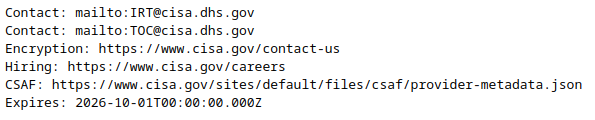
\includegraphics[width=\linewidth]{../resources/images/cisa_securitytxt.png}
  \captionof{figure}{
  The US Cybersecurity and infrastructure Agency (CISA) \texttt{security.txt} file.
  }
  \label{fig:cisa_securitytxt}
  \end{minipage}
  \end{center}

\vspace{1em}Congruent with RFC 9116 and the CISA guidance, the scanner sends a \texttt{GET} request to the paths '\texttt{/security.txt}', and '\texttt{/.well-known/security.txt}'.
A response is considered a candidate \texttt{security.txt} file if the server returns 200 OK and the response contains at least one \texttt{Contact:} field or a 
syntactically valid \texttt{Expires:} field that exist in the future at scan time. Lastly, the scanner parses whether any canonical URLs are listed. This evaluation
is scoped at the origin, as each server may contain the \texttt{security.txt} resources at different URIs.

\subsubsection{Security Headers \& Cookies}

\vspace{1em}Additionally, our scanner also performs a series of presence and evaluation checks on set of security headers. These checks are performed on 
each of the final URIs (URI-scoped). First we record the presence of the \texttt{Referrer-Policy} header.
The \texttt{Referrer-Policy} header controls how much of the current page's URL (the ``referrer'') is sent 
along when a browser navigates to another site or loads third-party content.
Without an explicit policy, browsers may send the full URL, including path and query parameters, 
to external services. 
On public-sector and financial sites, these URLs can easily contain case identifiers or other sensitive information. 
We derive this header's evaluation from the guidance
of OWASP and MDN. 

% OWASP recommends setting the header to \texttt{Referrer-Policy: strict-origin-when-cross-origin} 
% \cite{owasp_http_security_response_headers}. This directive
% indicates the browser should only send the origin, path, and query string when making a same-origin request, only send the origin
% in cross-origin requests when protocol security remains the same (e.g., HTTPS to HTTPS), and finally never send the \texttt{Referer} header to less secure destinations (e.g., HTTPS to HTTPS). 
% MDN advocates for setting the strictest \texttt{Referrer-Policy} comptable with th server. MDN lists the following derictives as the only \emph{client-protecting} directives in
% decreasing order of protection; \texttt{no-referrer}, \texttt{no-origin}, \texttt{strict-origin}, \texttt{strict-origin-when-cross-origin} 
% \cite{mdn_referrer_policy_config}. 
% Following OWASP and MDN guidance, we treat policies that never send full paths to third-party origins (for example \texttt{strict-origin-when-cross-origin}, 
% \texttt{strict-origin}, \texttt{same-origin}, or \texttt{no-referrer}) as recommended defaults 
% . Policies that still expose full URLs across sites (such as \texttt{unsafe-url} or \texttt{origin-when-cross-origin}) are classified as weak. Absense of the policy
% is also treated as recommended, since MDN states the default is \texttt{strict-origin-when-cross-origin}.


% \vspace{1em}Attackers can sometimes load a legitimate government or banking page inside a hidden 
% \texttt{<iframe>} and trick a user into clicking on real buttons (for example ``Approve payment'' or 
% ``Submit application'') 
% while believing they are interacting with a harmless overlay. 
% To counter this ``clickjacking'' risk, modern guidance recommends
% setting the \texttt{X-Frame-Options} header. In line with this guidance, the 
% scanner records the presence of the {X-Frame-Options} header.

% that restricts 
% framing (for example \texttt{frame-ancestors 'none'} or \texttt{frame-ancestors 'self'}) and 
%whether it sets \texttt{X-Frame-Options}
% to \texttt{DENY} or \texttt{SAMEORIGIN}. Configurations that completely forbid framing 
%(\texttt{'none'} or \texttt{DENY}) are treated
% as recommended; policies that only allow the site's own pages to frame themselves (\texttt{'self'} or 
%\texttt{SAMEORIGIN}) are treated 
% as acceptable but weaker. Sites that omit both controls, or explicitly allow any domain to frame
% them, are classified as lacking clickjacking protection.

% \vspace{1em}The next header we evaluate is the \texttt{Content-Security-Policy} (CSP). The CSP aims at reducing the attack surface
% of cross-site scripting (XSS) and other content-injection attacks by restricting which sources of scripts, images, and 
% other resources the browser may load. Consider the following illustrative example of an XSS attack: a bad actor discovers a 
% vulnerable input field on a government services page and injects a malicious \texttt{<script>} tag that 
% attempts to steal session
% cookies or redirect users to a phishing site. Without a restrictive CSP, the browser would execute this injected script. 
% With a proper CSP in place, however, the browser blocks the untrusted script, preventing the attack from succeeding even if an 
% injection point exists. The MDN, OWASP and UK Government Digital Services (GDS) all recommend setting an explicit CSP 
% \cite{mdn_csp_guide, owasp_csp_cheatsheet,gds_security_overview_websites}.  Policies that explicitly forbid all framing 
% (e.g.\ \texttt{frame-ancestors 'none'}) are classified as \emph{recommended}. Policies that allow only the 
% site itself (and any explicitly named partners) to frame the content (e.g.\ \texttt{frame-ancestors 'self' 
% https://example.gov}) are classified as \emph{sufficient}. If the CSP header is missing altogether, does not 
% define \texttt{frame-ancestors}, or uses a wildcard (e.g.\ \texttt{frame-ancestors *}), we classify the site 
% as \emph{insecure} for the purpose of clickjacking protection. Any other patterns are recorded but treated as 
% \emph{unknown} rather than over-interpreted. This aims to answer the question: 
% ``Are sites explicitly controlling who can embed their content?''.

\vspace{1em}The next header we evaluate is the \texttt{Content-Security-Policy} (CSP). The CSP aims at reducing the 
attack surface of cross-site scripting (XSS) and other content-injection attacks by restricting which 
sources of scripts, images, and 
other resources the browser may load. Providing additional security over the aforementioned 
\texttt{X-Frame-Options}.
The MDN, OWASP and UK Government Digital Services (GDS) all recommend setting an 
explicit CSP 
\cite{mdn_csp_guide, owasp_csp_cheatsheet,gds_security_overview_websites, owasp_clickjacking_defense} with 
the \texttt{frame-ancestors} directive. This directive controls exactly which other origins are 
allowed to embed this origin's content inside an \texttt{<iframe>}.
CSP is a powerful but application specific measure, we therefore interpret our CSP results narrowly, 
focusing on \texttt{Content-Security-Policy: frame-ancestors} directive.
The scanner records whether a response includes a \texttt{Content-Security-Policy} header and, if so, 
whether it contains \texttt{frame-ancestors} directive.

% we therefore interpret our CSP results narrowly, focusing on \texttt{Content-Security-Policy: frame-ancestors} directive.
% This directive provides defence against an attack known as ``clickjacking''. Clickjacking refers to when a malicious website
% embeds another website inside an invisible \texttt{<iframe>}. Thus tricking the user into taking potentially harmful actions
% unknowlingly. OWASP recommends setting the \texttt{frame-ancestors} derective to control exactly which other origins are 
% allowed to embed this origin's content inside an \texttt{<iframe>} \cite{owasp_clickjacking_defense}. 
% As such, we record whether a response includes a 
% \texttt{Content-Security-Policy} header and, if so, 
% extract and classify its \texttt{frame-ancestors} directive. Policies that explicitly forbid all framing 
% (e.g.\ \texttt{frame-ancestors 'none'}) are classified as \emph{recommended}. Policies that allow only the 
% site itself (and any explicitly named partners) to frame the content (e.g.\ \texttt{frame-ancestors 'self' 
% https://example.gov}) are classified as \emph{sufficient}. If the CSP header is missing altogether, does not 
% define \texttt{frame-ancestors}, or uses a wildcard (e.g.\ \texttt{frame-ancestors *}), we classify the site 
% as \emph{insecure} for the purpose of clickjacking protection. Any other patterns are recorded but treated as 
% \emph{unknown} rather than over-interpreted. This aims to answer the question: 
% ``Are sites explicitly controlling who can embed their content?''.

% Consider the following illustrative example of an XSS attack: a bad actor 
% discovers a 
% vulnerable input field on a government services page and injects a malicious \texttt{<script>} tag that attempts 
% to steal session
% cookies or redirect users to a phishing site. Without a restrictive CSP, the browser would execute this injected script. 
% With a proper CSP in place, however, the browser blocks the untrusted script, preventing the attack from succeeding 
% even if an 
% injection point exists. 

% \vspace{1em}
% An older security header that aims to reduce the risk of clickjacking is 
% \texttt{X-Frame-Options} (XFO). Although largely superseded by the 
% \texttt{frame-ancestors} directive in CSP, many sites still rely on XFO
% for backwards compatability. Similar to the CSP's \texttt{frame-ancestors} derective, XFO instructs the 
% browser whether the page may be 
% displayed inside a \texttt{<frame>} or \texttt{<iframe>} element. The header 
% supports three directives: \texttt{DENY} (never permit framing), 
% \texttt{SAMEORIGIN} (allow framing only by pages from the same site), and 
% \texttt{ALLOW-FROM <origin>}. Our scanner attempts to retrieve the raw XFO header. If the header is present and set to 
% \texttt{DENY}, we classify the site as \emph{recommended}. If set to 
% \texttt{SAMEORIGIN}, we classify it as \emph{sufficient}, since the site at 
% least restricts framing to itself. If the site sets XFO to \texttt{ALLOW-FROM}, we record this as \emph{obsolete}---as this directive is now deprecated. 
% If the header is missing entirely, contains unknown syntax, or is malformed we treat it as \emph{unknown}.

\vspace{1em}The \texttt{X-Content-Type-Options} header is a simple but important control. This header eliminates 
``MIME Sniffing'', where a browser may \emph{guess} the MIME (Multipurpose Internet Mail Extension) type of a 
resource and act accordingly. This behaviour can be abused in so-called MIME confusion
attacks, where user-supplied or third-party content is interpreted as active HTML or JavaScript instead of 
static data. OWASP recommends administrators to set the \texttt{X-Content-Type-Options} to \texttt{nosniff}, instructing
the browser to \emph{always} follow the content type found in the \texttt{Content-Type} header
\cite{owasp_http_security_response_headers, mdn_mime_types_guide}. In line with OWASP's guidance, the scanner records
the presence of \texttt{X-Content-Type-Options} in the response of the final resolved URI.

% In line with this guidance, 
% our scanner performs a simple
% check as to whether the endpoint has the \texttt{X-Content-Type-Options} header present, and 
% whether it's value is set
% to \texttt{nosniff}.

\vspace{1em}The next header the scanner records is the \texttt{Permissions-Policy} (formerly \texttt{Feature-Policy}). This header allows a site
to declare which powerful browser features are enabled on a page and which embedded origins, if any, may use them. Examples include 
access to the camera, microphone, geolocation, clipboard and more. 
In the absence of an explicit policy, browsers generally assume that these features are available to the top-level origin and depending on the feature, 
embedded third-party content. Both OWASP and Google Chrome both recommend web administrators explicitly set the \texttt{Permissions-Policy} 
\cite{owasp_http_security_response_headers, chrome_permissions_policy}, 
disabling what isn't in use. 

% The scanner checks for this response header, and 
% evaluates whether this endpoint is explicitly controlling certain features via structured directives of the form 
% \texttt{feature = sources}(e.g., \texttt{camera=()})

\vspace{1em}Cookies are a common mechanism for tracking sessions and user state on the web. 
Even ostensibly ``public'' pages often set cookies for language preferences, analytics, or short-lived 
session identifiers. Due to cookies being sent automatically to a site with each request, weak cookie settings can expose
users to eavesdropping, cross-site request forgery (CSRF), or theft of authentication tokens. The CCCS 
explicitly recommends the use of cookie security flags as part of secure session
management \cite{cccs_itsp_40_111}. Additionally, MDN provides practical guidance on applying these flags in modern 
applications \cite{mdn_secure_cookie_configuration}. Furthermore, OWASP marks multiple cookie protection mechanisms as mandatory.
In particular, three attributes are widely recognized as baseline protections:
\begin{itemize}
  \item \textbf{\texttt{Secure}} ensures that a cookie is only sent over HTTPS, preventing passive attackers on the network from reading its value on unencrypted connections.
  \item \textbf{\texttt{HttpOnly}} prevents JavaScript from accessing the cookie via \texttt{document.cookie}, which limits the impact of cross-site scripting (XSS) attacks on session tokens.
  \item \textbf{\texttt{SameSite}} limits when cookies are sent on cross-site requests. Strict or lax settings here can significantly reduce CSRF state changes by omitting cookies from certain cross-origin operations.
\end{itemize}

To evaluate how these protections are used in practice, our scanner inspects the \texttt{Set-Cookie} header on the final 
landing page and parses any attributes attached to each cookie name–value pair. We record whether the \texttt{Secure} and 
\texttt{HttpOnly} flags are present, the value of the \texttt{SameSite} attribute (if any), and whether
 the cookie appears to have an explicit lifetime via \texttt{Max-Age} or \texttt{Expires}. 
Because some informational sites do not set 
cookies at all, we only apply this check when at least one \texttt{Set-Cookie} header is observed on the 
landing page. For the purposes of this study, cookies that are marked both \texttt{Secure} and \texttt{HttpOnly} and use a 
strict
\texttt{same-site} policy are classified as \emph{recommended}, 
reflecting CCCS, MDN and OWASP guidance for session management. 
Cookies that are \texttt{Secure} and \texttt{HttpOnly} but use a more permissive same-site setting 
(e.g., \texttt{SameSite=Lax}) are treated as \emph{sufficient}, 
since they still provide substantial protection against token theft and many cross-site attacks. 
Cookies that lack any of these flags, particularly those that are neither \texttt{Secure} nor \texttt{HttpOnly} 
or that omit a same-site policy entirely, are classified as \emph{insecure}. 

\subsubsection{Information Leakage}

\vspace{1em}Beyond checking for the presence of modern security headers, we also examined whether sites leaked 
unnecessary implementation details through so--called 
``revealing'' HTTP response headers. This check once again targets the final URI. 
These are headers that advertise the underlying web server, framework, CMS, or platform. Prior work by the OWASP 
HTTP Security Response Headers
Cheat Sheet and the OWASP Secure Headers Project explicitly recommends removing or genericising headers such as 
\texttt{Server}, \texttt{X-Powered-By}, 
and framework version banners because they ease fingerprinting and targeted exploitation of known vulnerabilities 
\cite{owasp_secure_headers_project, owasp_http_security_response_headers}. 
More generally, government and national guidance on secure configuration, including CCCS ITSG--33 and related profiles, emphasises limiting information leakage from public services, 
which includes avoiding unnecessary disclosure of software and version details. To operationalize this, our scanner 
imported OWASP Secure Headers Project's list of ``revealing'' headers \cite{owasp_secure_headers_remove_json}. 
For each origin's final response, the scanner recorded whether any response header name matched the OWASP list 
(e.g., \texttt{server}, \texttt{x-powered-by}, etc.), and whether that response header contained version leaks.

% \begin{table}[h]
%   \centering
%   \begin{tabular}{p{3cm}p{4.5cm}p{6.5cm}}
%     \hline
%     \textbf{Header} & \textbf{Example value} & \textbf{Why it is revealing} \\
%     \hline
%     \texttt{Server} &
%     \texttt{Apache/2.4.49 (Unix)} &
%     Discloses the exact web server product and version; attackers can search for this version when a remote code execution or path traversal CVE is published. \\
%     \texttt{X-Powered-By} &
%     \texttt{PHP/7.4.33} or \texttt{Express} &
%     Reveals the application platform or framework in use (PHP, Node.js, etc.), again often with a specific version number. \\
%     \texttt{X-Generator} &
%     \texttt{Drupal 9.4.1}, \texttt{PrestaShop} &
%     Discloses the CMS product and version, facilitating targeted CMS exploitation. \\
%     \hline
%   \end{tabular}
%   \caption{Examples of ``revealing'' HTTP headers tracked by our scanner. These headers are not required for end-user functionality but expose details about the server's software stack and versions. Our analysis focuses on how many public-sector sites retain such headers versus those that follow OWASP guidance and remove or genericise them.}
%   \label{tab:revealing-headers-examples}
% \end{table}


\vspace{1em}Misconfigured error pages are another common source of unintended information disclosure 
\cite{owasp_top10_a05_2021,owasp_error_handling,cwe_209}. These error pages can reveal the exact framework, cloud provider, or 
database in use, and in the worst case they display full stack traces to unauthenticated users. Since leaks occur at the web application level, we perform this evaluation
on origins. To assess this risk in a safe and consistent way, we carried out a
single, non-invasive probe of each origin's error handling. For every origin, the scanner issued one HTTPS \texttt{GET} request to a deliberately non-existent path of the form 
\texttt{https://\textit{origin}/\_\_scanner\_404\_\_\textit{token}/}, where \textit{token} is a 
random 16-character string chosen per origin. This is
intended to trigger the site's standard 404/4xx error handler without sending any exploit payloads. 
Responses were only analysed further if the \texttt{Content-Type} header indicated textual 
content. 
Otherwise, the origin was treated as not exposing any interpretable error page. The body of each error page was then scanned for two classes of
information leaks. First, we looked for technology banners using a curated set of signatures for common web frameworks, cloud platforms, and databases. These signatures
were derived from the most widely used web technologies in the 2025 Stack Overflow Developer Survey \cite{stackoverflow_survey_2025}. 
Each technology's alias was compiled into a case-insensitive regular expression (REGEX) that escapes punctuation, tolerates 
minor formatting differences, and provides simple word-boundary semantics using negative look-behind/ahead. Thus, allowing the scanner to match whole 
identifiers (e.g., django or django 4.2.5) but not substrings inside longer words.

\vspace{1em}Second, we scanned each error page for stack traces from widely used backend languages, sourced from the previously mentioned Stack Overflow Developer Survey. For
each language we defined a pair of regular-expression families. These families include header patterns
that identify the start of a stack trace (e.g., ``\texttt{Traceback (most recent call last):}'') and frame patterns that match subsequent call-site lines. 
When the header of a trace was found, we looked ahead through a number of lines to count how many frames followed. If at least one frame was detected, 
the leaked language is recorded. Results were limited to at most one trace per language per origin.

\subsection{Scanner Implementation \& Validation}

\vspace{1em}To keep our scan non-invasive and respectful, the scanner was built to allow a configured 
total and per-origin simultaneous connection limit. 
For the authority sites, we allowed 15 total concurrent connections, with at most 
3 connections to each origin at a time. For other sectors (finance, education, energy) 
we allowed 20 total concurrent connections with 5 concurrent per origin. Each request was bounded by a client-side timeout of 3 seconds. 
The scanner also maintains per-origin timeout counters.
Origins that accumulated 3 HTTP timeouts or 2 TLS timeouts were marked as temporarily dead for that protocol, 
and no further HTTP/TLS modules were run against them. These hyper-conservative constraints were chosen to ensure ethical scanning practice 
and prevent service disruption. Thus, allowing us to distinguish genuinely unreachable sites, 
without inundating servers with excessive traffic.


\vspace{1em}Because our conclusions depend on automated classification, we invested effort in testing the scanner 
itself
before running it at scale. The goal of these tests was not to prove the scanner is perfect, but to ensure that, 
for a wide range of realistic inputs, the implementation behaves in a way that matches the methodology described above.
First, we built automated tests for individual modules such as target parsing, HTTPS/TLS connectivity, security.txt 
discovery and 
header classification. For these tests we spun up small local web servers on \texttt{localhost} with controlled behaviour
 (e.g., specific redirects, header combinations, or security.txt contents) and ran the scanner against them. This 
allowed us to verify that each module correctly interpreted well-formed responses, handled missing or malformed fields 
gracefully, 
and produced the expected results for the security headers and cookie flags. 
TLS-related tests were performed against local HTTPS endpoints using self-signed certificates. 
We confirmed that the scanner correctly distinguished between successful and failed HTTPS connections by 
varying certificate properties and connection parameters on the local web servers. 

\vspace{1em}To validate the scanner's error leak detection, we first tested the regular-expression approach offline. 
For each web language, we intentionally executed failing code to 
generate genuine stack traces and error pages in that language's default format. These raw error messages were 
fed directly into the parser to confirm that the scanner reliably detected the expected language/technology and 
extracted the 
correct label. In parallel, we ran the same detector over leak-free HTML and JSON data drawn from real web endpoints. Asserting that 
no stack traces or banners were reported, thus guarding against false positives. Similar to the previous tests, we then configured small local web servers to return known responses on specific paths, including pages that 
contained the captured error messages or only normal content. The scanner then scanned these local endpoints, and our tests 
asserted the same results were recorded over HTTP. 

\vspace{1em}Finally, we ran end-to-end tests in which all modules were exercised together, imitating a small scan 
from input list to
aggregated results. In these scenarios, the scanner was pointed at a collection of local test servers designed to emulate a mix of 
secure, partially configured and clearly misconfigured sites. We then compared the resulting findings against an expected 
``ground truth'' for each test target. 



% \subsection{Data Analysis}
% % Data analysis plan:
% % - For each site, derive binary/ternary indicators per check:
% %   * Example: HTTPS enforced (yes/no/partial), HSTS quality (good/weak/missing), TLS version support (modern/legacy), etc.
% % - Aggregate by:
% %   * Sector (authority/finance/education/energy).
% %   * Jurisdiction (CA/US/UK).
% %   * CDN/WAF vs non-CDN (where inferable from headers/CNAMEs).
% % - Compute:
% %   * Proportion of sites meeting each recommended control.
% %   * "Profiles" of controls (e.g., % with strong TLS but weak headers vs the reverse).
% %   * Distribution of security.txt adoption, CSP presence, and cookie flag hygiene.
% % - For RQ2:
% %   * Compare distributions across CA vs US vs UK for the same sector.
% %   * Highlight statistically meaningful gaps (even if just descriptive comparisons, not heavy stats).
% % - Handle WAF-affected sites:
% %   * Treat as a distinct category (unmeasurable due to active blocking).
% %   * Report their counts separately to avoid biasing denominators.

% \subsection{Evaluation metrics}
% % Evaluation metrics:
% % - Per-check classification:
% %   * Recommended / acceptable / missing, based on concrete standards (e.g., HSTS max-age >= 1 year; TLS >= 1.2; Referrer-Policy at least strict-origin-when-cross-origin; etc.).
% % - Site-level "profiles" instead of a single score:
% %   * Transport posture: {modern TLS only, legacy allowed, HTTPS not enforced}.
% %   * Header posture: {all key hardening headers present, partial, minimal}.
% %   * Application posture: {no error leaks, minor leaks, stack trace / directory listing exposed}.
% %   * Disclosure posture: {security.txt present and complete, present but weak, absent}.
% % - Sector/jurisdiction metrics:
% %   * For each sector + jurisdiction: report percentages for all major checks with CIs or at least clear N.
% % - Optional composite:
% %   * A simple "meets a minimum Canadian baseline" flag (e.g., HTTPS enforced, HSTS present, modern TLS only, no obvious error leaks) to answer RQ1 succinctly.


\section{Results}\label{sec:result}

\subsection{URL \& Origin Normalization}

The table below illustrates the outcome of our initial resolution stage. The columns represent the
number of input URIs, distinct final URIs and final origins after following
redirects, and the percentage of inputs that ended in a successful 2xx
response, a final 4xx/5xx response, or no final URL. Plus the percentage
of origins whose inputs were all unreachable from the scanner's vantage point. 

\begin{inlinecap}  % no argument; default is \textwidth
  \captionof{table}{Redirect resolution outcomes by country and sector.}
  \label{tab:redirect_summary}
  \centering
  \scriptsize
  \setlength{\tabcolsep}{2.5pt}
  \resizebox{\textwidth}{!}{%
    \csvreader[
      tabular=lllrrrrrrrr,  % Added one more 'r' column
      table head=\toprule
        Dataset & Sector &
        $n$ URIs &
        $n$ final URIs &
        $n$ input origins &
        $n$ final origins &
        $n$ unique final origins &  % NEW COLUMN
        Final 2xx (\%) &
        Final 4xx/5xx (\%) &
        No final URL (\%) &
        Origins all unreachable (\%) \\\midrule,
      late after line=\\,
      late after last line=\\\bottomrule
    ]{../results/comparison/redirects/redirects_summary.csv}{%
      dataset_label=\Dataset,
      sector_label=\Sector,
      n_input_uris=\Nuris,
      n_final_uris=\Nfuri,
      n_input_origins=\Niorig,
      n_final_origins=\Nforig,
      pct_final_2xx=\P2xx,
      pct_final_4xx_5xx=\Perr,
      pct_no_final=\Pno,
      pct_origins_all_unreachable=\PorigDead
    }{%
      \Dataset & \Sector &
      \Nuris & \Nfuri & \Niorig & \Nforig &
      % NEW: Conditional column for n unique final origins
      \ifnum\pdfstrcmp{\Dataset}{CA Authorities}=0 375\fi%
      \ifnum\pdfstrcmp{\Dataset}{CA Education}=0 103\fi%
      \ifnum\pdfstrcmp{\Dataset}{CA Finance}=0 157\fi%
      \ifnum\pdfstrcmp{\Dataset}{CA Energy}=0 188\fi%
      \ifnum\pdfstrcmp{\Dataset}{US Authorities}=0 373\fi%
      \ifnum\pdfstrcmp{\Dataset}{US Education}=0 53\fi%
      \ifnum\pdfstrcmp{\Dataset}{US Finance}=0 107\fi%
      \ifnum\pdfstrcmp{\Dataset}{US Energy}=0 141\fi%
      \ifnum\pdfstrcmp{\Dataset}{UK Authorities}=0 4\fi%
      \ifnum\pdfstrcmp{\Dataset}{UK Education}=0 447\fi%
      \ifnum\pdfstrcmp{\Dataset}{UK Finance}=0 165\fi%
      &  % End of new column
      \P2xx & \Perr & \Pno & \PorigDead
    }%
  }%
  \end{inlinecap}

\vspace{1em}Among Canadian authority inputs, 68.4\% resolved to final 2xx responses, 5.2\% ended in 
4xx/5xx errors, and 26.4\% failed to reach any final URL due to timeouts or connection 
failures. The 342 input origins expanded to 238 final origins after redirect resolution, 
with 18.6\% of origins completely unreachable. US authorities showed comparable patterns 
with 72.4\% success, 27.2\% no final URL, and 21.7\% completely unreachable origins. 
UK authorities achieved 88.0\% successful resolution but represent only 3 input origins 
expanding to 3 final origins.

\subsection{Website Security Evaluation}

\subsubsection{Transport Security}

\vspace{1em}Following redirect resolution, we outline the results of our HTTPS redirection, and HSTS probes. 
We compare each sector of each country against the Canadian authority sites. Across the 
373 Canadian authority origins, roughly three quarters (73\%) successfully served a page over 
HTTPS from our vantage point, while about one quarter returned HTTPS errors or were unreachable. 
Over HTTP, almost all origins responded (94\%), and nearly nine in ten  ($\approx89\%$) 
redirected users to HTTPS, with only a small minority either serving a non-redirecting HTTP 
page or redirecting somewhere other than HTTPS. 
Among HTTPS-capable sites, almost nine in ten deployed HSTS at all, and about two-thirds of 
those used a ``strong'' policy (at least one-year max-age with includeSubDomains), 
often with the preload flag set. Note that the ``unreachable'' column in this table is \emph{not} 
an indicator that the site is offline. Rather, ``unreachable''  that
our scanner was repeatedly unable to complete a TLS handshake or receive an HTTP response. 
This behaviour suggests bot mitigation, rate limiting, or WAF/CDN filtering---not unavailability.

\begin{inlinecap}
\captionof{table}{HTTP/HTTPS connectivity outcomes by country and sector.
Values are the percentage of origins in each dataset that successfully served HTTPS,
were unreachable over HTTPS, responded to an HTTP probe at all, redirected HTTP to HTTPS,
or served HTTP without redirecting.}
\label{tab:https_connectivity}
\centering
\scriptsize
\setlength{\tabcolsep}{2.5pt}
\resizebox{\textwidth}{!}{%
\csvreader[
  tabular=llrrrrrr,
  table head=\toprule Dataset & Sector &
    $n$ origins &
    HTTPS ok (\%) &
    HTTPS unreachable (\%) &
    HTTP probe ok (\%) &
    HTTP$\to$HTTPS redirect (\%) &
    HTTP no redirect (\%) \\\midrule,
  late after line=\\,
  late after last line=\\\bottomrule
]{../results/comparison/https_hsts/https_hsts_enforcement_summary.csv}{%
  dataset_label=\Dataset,
  sector_label=\Sector,
  n_origins=\Norigins,
  pct_https_success=\PHttpsOk,
  pct_https_unreachable=\PUnreach,
  pct_http_probe_ok=\PHttpOk,
  pct_http_redirect_to_https=\PRedir,
  pct_http_no_redirect=\PNoRedir
}{%
  \Dataset & \Sector &
  \Norigins & \PHttpsOk & \PUnreach & \PHttpOk & \PRedir & \PNoRedir
}%
}%
\end{inlinecap}

% \begin{inlinecap}
% \captionof{table}{HTTPS reachability and HSTS configuration quality by country and sector.
% For each dataset we report the number of origins that successfully served HTTPS and, among
% those, the share that enabled HSTS at all, used a strong HSTS policy, and included
% a long max-age, subdomain coverage, and the preload flag.}
% \label{tab:https_hsts_quality}
% \centering
% \scriptsize
% \setlength{\tabcolsep}{2.5pt}
% \resizebox{\textwidth}{!}{%
%   \csvreader[
%     tabular=llrrrrrrr,
%     table head=\toprule Dataset & Sector &
%       $n$ HTTPS ok &
%       $n$ with HSTS &
%       Any HSTS (\% of HTTPS ok) &
%       Strong HSTS (\% of HSTS) &
%       HSTS max-age $\geq$ 1y (\% of HSTS) &
%       HSTS incl.\ subdom.\ (\% of HSTS) &
%       HSTS preload flag (\% of HSTS) \\\midrule,
%     late after line=\\,
%     late after last line=\\\bottomrule
%   ]{../results/comparison/https_hsts/hsts_quality_summary.csv}{%
%     dataset_label=\Dataset,
%     sector_label=\Sector,
%     n_https_ok=\NHttpsOk,
%     n_has_hsts=\NHasHsts,
%     pct_has_hsts_among_https_ok=\PAnyHsts,
%     pct_hsts_strong_among_hsts=\PStrong,
%     pct_hsts_maxage_1yr_among_hsts=\PMaxAge,
%     pct_hsts_include_subdomains_among_hsts=\PSubs,
%     pct_hsts_preload_among_hsts=\PPreload
%   }{%
%     \Dataset & \Sector &
%     \NHttpsOk & \NHasHsts &
%     \PAnyHsts & \PStrong & \PMaxAge & \PSubs & \PPreload
%   }%
% }%
% \end{inlinecap}

\begin{inlinecap}
  \captionof{table}{HTTPS reachability and HSTS configuration quality by country and sector.
  For each dataset we report the number of origins that successfully served HTTPS and, among
  those, the share that enabled HSTS at all, used a strong HSTS policy, and included
  a long max-age, subdomain coverage, and the preload flag.}
  \label{tab:https_hsts_quality}
  \centering
  \scriptsize
  \setlength{\tabcolsep}{2.5pt}
  \resizebox{\textwidth}{!}{%
    \csvreader[
      tabular=llrrrrrrr,
      table head=\toprule
        \multicolumn{2}{c}{Dataset} &
        \multicolumn{2}{c}{Counts} &
        \multicolumn{5}{c}{Share of sites (\%)} \\
        \cmidrule(lr){1-2}\cmidrule(lr){3-4}\cmidrule(l){5-9}
        Dataset & Sector &
        $n$ HTTPS ok &
        $n$ with HSTS &
        Any HSTS (of HTTPS ok) &
        Strong HSTS (of HSTS) &
        max-age $\geq$ 1y (of HSTS) &
        incl.\ subdom.\ (of HSTS) &
        preload flag (of HSTS) \\\midrule,
      late after line=\\,
      late after last line=\\\bottomrule
    ]{../results/comparison/https_hsts/hsts_quality_summary.csv}{%
      dataset_label=\Dataset,
      sector_label=\Sector,
      n_https_ok=\NHttpsOk,
      n_has_hsts=\NHasHsts,
      pct_has_hsts_among_https_ok=\PAnyHsts,
      pct_hsts_strong_among_hsts=\PStrong,
      pct_hsts_maxage_1yr_among_hsts=\PMaxAge,
      pct_hsts_include_subdomains_among_hsts=\PSubs,
      pct_hsts_preload_among_hsts=\PPreload
    }{%
      \Dataset & \Sector &
      \NHttpsOk & \NHasHsts &
      \PAnyHsts & \PStrong & \PMaxAge & \PSubs & \PPreload
    }%
  }%
  \end{inlinecap}
  

The following table summarizes TLS protocol support, naturally negotiated versions, and forced TLS 1.2 cipher quality across 
all datasets for each country and sector. 
For each origin, we probed which TLS protocol versions (1.0, 1.1, 1.2, 1.3) the server advertises support for. Following this recorded the 
version and cipher suite negotiated during a standard handshake, and then performed forced TLS 1.2 handshakes to 
classify cipher suites into recommended, sufficient, phase-out, insecure, or unknown 
categories based on CCCS guidance.
    
\begin{inlinecap}
  \captionof{table}{TLS protocol support, negotiated versions, and cipher categories by country and sector.}
  \label{tab:tls_cipher_summary}
  \centering
  \tiny
  \setlength{\tabcolsep}{1.5pt}
  \resizebox{\textwidth}{!}{%
    \csvreader[
      tabular=llrrrrrrrrrrrrrr,
      table head=\toprule
        Country & Sector & $n$ origins &
        \multicolumn{4}{c}{TLS Support (\%)} &
        \multicolumn{3}{c}{Negotiated (\%)} &
        \multicolumn{5}{c}{TLS 1.2 Cipher Categories (\%)} \\
        \cmidrule(lr){4-7} \cmidrule(lr){8-10} \cmidrule(lr){11-15}
        & & & 1.3 & 1.2 & 1.1 & 1.0 & 1.3 & 1.2 & Other & Rec. & Suff. & Phase & Insec. & Unk. \\\midrule,
      late after line=\\,
      late after last line=\\\bottomrule
    ]{../results/comparison/tls_cipher/tls_cipher_summary.csv}{%
      country=\Country,
      sector=\Sector,
      n_origins=\Norigins,
      pct_tls13_support=\TLSa,
      pct_tls12_support=\TLSb,
      pct_tls11_support=\TLSc,
      pct_tls10_support=\TLSd,
      n_with_version=\Nwv,
      pct_tls13_neg=\Nega,
      pct_tls12_neg=\Negb,
      pct_other_neg=\Negc,
      n_tls12_forced=\Ntf,
      pct_recommended=\Crec,
      pct_sufficient=\Csuf,
      pct_phase_out=\Cphs,
      pct_insecure=\Cins,
      pct_unknown=\Cunk
    }{%
      \Country & \Sector & \Norigins &
      \TLSa & \TLSb & \TLSc & \TLSd &
      \Nega & \Negb & \Negc &
      \Crec & \Csuf & \Cphs & \Cins & \Cunk
    }%
  }%
  \end{inlinecap}
  
The chart below illustrates the negotiated version of TLS recorded in a ``natural'' handshake. This handshake 
represents what a typical Canadian's user agent (browser) recieves in practice. We note here the Canadian authority
sites lower proclivity for negotiating TLS~1.3 (vs higher TLS~1.2) compared to the other sectors. 

  \begin{inlinecap}
    \label{fig:tls_stacked_auth_fin}
    \centering
    \scriptsize
    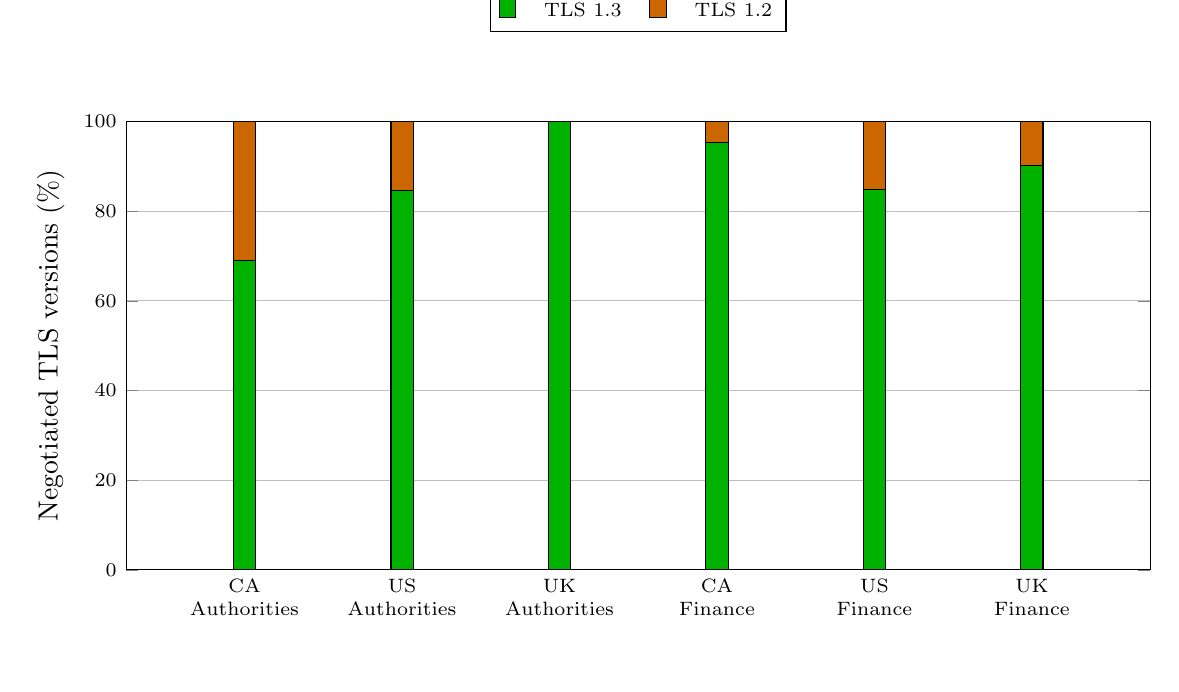
\begin{tikzpicture}
      \begin{axis}[
        ybar stacked,
        bar width=8pt,
        x=2cm,
        enlarge x limits=0.15,
        ymin=0, ymax=100,
        ylabel={Negotiated TLS versions (\%)},
        symbolic x coords={CA-Auth,US-Auth,UK-Auth,CA-Fin,US-Fin,UK-Fin},
        xtick=data,
        xticklabels={
          CA\\Authorities,
          US\\Authorities,
          UK\\Authorities,
          CA\\Finance,
          US\\Finance,
          UK\\Finance
        },
        xticklabel style={
          align=center,
          font=\scriptsize,
          text width=1.6cm
        },
        tick label style={font=\scriptsize},
        ymajorgrids=true,
        legend style={
          at={(0.5,1.20)},
          anchor=south,
          legend columns=3,
          column sep=8pt,
          font=\scriptsize,
        },
      ]
  
        \addplot[fill=green!70!black] coordinates {
          (CA-Auth, 69.1)
          (US-Auth, 84.6)
          (UK-Auth,100.0)
          (CA-Fin, 95.4)
          (US-Fin, 84.9)
          (UK-Fin, 90.2)
        };
  
        \addplot[fill=orange!80!black] coordinates {
          (CA-Auth, 30.9)
          (US-Auth, 15.4)
          (UK-Auth,  0.0)
          (CA-Fin,  4.6)
          (US-Fin, 15.1)
          (UK-Fin,  9.8)
        };
  
        \legend{TLS 1.3, TLS 1.2}
      \end{axis}
    \end{tikzpicture}
    \captionof{figure}{Stacked bar chart of negotiated TLS versions for authority and finance websites by country.}
  \end{inlinecap}

Among Canadian authority origins, 65.9\% advertised TLS 1.3 support and 94.4\% supported TLS 1.2, 
while 11.5\% still accepted TLS 1.1 and 9.6\% accepted TLS 1.0. During natural handshakes, 69.1\% of these authorities negotiated TLS 1.3 and 30.9\% negotiated TLS 1.2, with no 
origins falling back to older protocols. When forced to use TLS 1.2, 74.9\% of Canadian authorities selected recommended cipher suites, 1.7\% selected sufficient ciphers, 
3.4\% used phase-out ciphers, none used insecure ciphers, and 20.1\% negotiated ciphers not categorized in CCCS guidance.

\subsubsection{Vulnerability Disclosure}

\vspace{1em}The next table reports security.txt adoption and field completeness by country and sector. For each origin, we probed standard locations 
(/.well-known/security.txt and /security.txt) for the presence of a security.txt 
file per RFC 9116, then parsed present files to assess whether they included required Contact and Expires fields, and 
whether Expires dates remained valid.

\begin{inlinecap}
\captionof{table}{Security.txt adoption and field completeness by country and sector.}
\label{tab:securitytxt_summary}
\centering
\small
\setlength{\tabcolsep}{3pt}
\resizebox{\textwidth}{!}{%
\csvreader[
tabular=llllrrrrr,
table head=\toprule
Dataset & Country & Sector &
$n$ origins &
$n$ with security.txt &
Sites w/ security.txt (\%) &
Contact field (\%) &
Expires field (\%) &
Valid expires (\%) \\\midrule,
late after line=\\,
late after last line=\\\bottomrule
]{../results/comparison/securitytxt/securitytxt_summary.csv}{%
dataset_label=\Dataset,
country=\Country,
sector_label=\Sector,
n_origins=\Norigins,
n_with_securitytxt=\Nwith,
pct_sites_with_securitytxt=\Psites,
pct_with_contact_among_present=\Pcontact,
pct_with_expires_among_present=\Pexpires,
pct_valid_expires_among_expires=\Pvalid
}{%
\Dataset & \Country & \Sector &
\Norigins & \Nwith & \Psites & \Pcontact & \Pexpires & \Pvalid
}%
}%
\end{inlinecap}

Among Canadian authority origins, only 1.1\% (4 of 375) 
published a security.txt file. All four files included Contact information and Expires fields, 
though only 25\% had unexpired dates. US authorities showed higher adoption at 3.5\% (13 of 373), 
with 92.3\% of those including Expires fields and 83.3\% maintaining valid expiration dates. 

% \vspace{1em}Across Canadian sectors, energy demonstrated the highest adoption at 4.2\% (9 origins), 
% followed by education at 3.9\% 
% (4 origins), while finance showed minimal adoption at 0.6\% (1 origin). US sectors 
% displayed comparable patterns, with education at 
% 5.7\%, finance at 2.8\%, and energy at 0.7\%. UK education and finance sectors showed 
% substantially higher adoption rates of 
% 5.8\% and 12.1\% respectively, though field completeness varied with only 75\% of UK education
% files and 50\% of UK finance 
% files including Expires fields. 

\vspace{1em}The following 2 tables present security header adoption and 
cookie security flag usage across all datasets. For each successfully reached origin, 
we analyzed HTTP response headers to identify the presence of key security headers 
(\texttt{Referrer-Policy}, \texttt{X-Content-Type-Options}, 
\texttt{X-Frame-Options}, \texttt{Content-Security-Policy}, \texttt{Permissions-Policy}) and 
cookie security attributes (Secure, HttpOnly, SameSite flags).

% Security Headers Presence Table
\begin{inlinecap}
\captionof{table}{Security header adoption by country and sector.}
\label{tab:security_headers_presence}
\centering
\tiny
\setlength{\tabcolsep}{2pt}
\resizebox{\textwidth}{!}{%
\csvreader[
tabular=llllrrrrr,
table head=\toprule
  Dataset & Country & Sector &
  $n$ sites &
  Referrer-Policy (\%) &
  X-Content-Type-Options (\%) &
  X-Frame-Options (\%) &
  CSP frame-ancestors (\%) &
  Permissions-Policy (\%) \\\midrule,
late after line=\\,
late after last line=\\\bottomrule
]{../results/comparison/headers/security_headers_presence.csv}{%
dataset_label=\Dataset,
country=\Country,
sector_label=\Sector,
n_sites=\Nsites,
pct_referrer_policy_present=\Pref,
pct_x_content_type_options_present=\Pxcto,
pct_x_frame_options_present=\Pxfo,
pct_csp_frame_ancestors_present=\Pcsp,
pct_permissions_policy_present=\Pperm
}{%
\Dataset & \Country & \Sector &
\Nsites & \Pref & \Pxcto & \Pxfo & \Pcsp & \Pperm
}%
}%
\end{inlinecap}

Overall, Canadian authorities show modest but uneven security-header adoption: 
simple headers are common, but usage drops sharply for more complex policies. 
US and UK authorities perform noticeably better, and within Canada the education sector generally 
outperforms authorities.

% Canadian authorities showed modest security header adoption, with 62.3\% 
% deploying X-Content-Type-Options, 64.5\% using \texttt{X-Frame-Options}, 17.9\% implementing CSP 
% frame-ancestors, 17.4\% setting \texttt{Referrer-Policy}, and only 8.6\% adopting \texttt{Permissions-Policy}. 
% US authorities outperformed across most headers, achieving 78.0\% for \texttt{X-Content-Type-Options}, 
% 81.2\% for \texttt{X-Frame-Options}, and 34.7\% for CSP frame-ancestors. UK authorities demonstrated
% substantially higher adoption at 87.7\% for X-Content-Type-Options and X-Frame-Options, 
% though this represents a small sample of 348 sites. Among Canadian sectors, education 
% consistently exceeded authorities' performance (60.4\% X-Content-Type-Options, 28.6\% 
% CSP frame-ancestors), while finance and energy showed mixed results with finance achieving 
% the highest Referrer-Policy adoption at 28.0\%.

\begin{inlinecap}
\captionof{table}{Cookie security flag adoption by country and sector.}
\label{tab:cookie_security_flags}
\centering
\small
\setlength{\tabcolsep}{3pt}
\resizebox{\textwidth}{!}{%
\csvreader[
tabular=llllrrrrr,
table head=\toprule
  Dataset & Country & Sector &
  $n$ sites &
  Sites w/ cookies (\%) &
  Secure flag (\%) &
  HttpOnly flag (\%) &
  SameSite$\ge$Lax (\%) &
  Rec./Suff. (\%) \\\midrule,
late after line=\\,
late after last line=\\\bottomrule
]{../results/comparison/headers/cookie_security_flags_summary.csv}{%
dataset_label=\Dataset,
country=\Country,
sector_label=\Sector,
n_sites=\Nsites,
pct_sites_with_cookies=\Pcookies,
pct_secure_among_cookie_sites=\Psecure,
pct_httponly_among_cookie_sites=\Phttp,
pct_samesite_ge_lax_among_cookie_sites=\Psame,
pct_rec_suff_among_cookie_sites=\Prec
}{%
\Dataset & \Country & \Sector &
\Nsites & \Pcookies & \Psecure & \Phttp & \Psame & \Prec
}%
}%
\end{inlinecap}  

Among Canadian authority origins setting cookies (28.2\% of all origins), 63.5\% used the 
Secure flag, 48.7\% used HttpOnly, 15.7\% implemented SameSite at Lax or Strict, and only 
3.5\% achieved recommended or sufficient configurations (Secure + HttpOnly + SameSite Strict/Lax). 
Canadian energy sites showed stronger cookie security with 74.4\% using Secure and 76.8\% 
using HttpOnly, achieving 4.9\% recommended configurations. US authorities showed comparable
patterns with 51.6\% Secure, 44.0\% HttpOnly, and 3.3\% recommended. While UK authorities' 
limited cookie-setting origins (0.6\% of 348 sites, or approximately 2 origins) 
achieved perfect flag implementation but represent insufficient data for meaningful comparison.

\subsubsection{Information Leakage}

% Revealing Headers Summary Table
\begin{inlinecap}
\captionof{table}{Distribution of technology-revealing headers by country and sector.}
\label{tab:revealing_headers_summary}
\centering
\small
\setlength{\tabcolsep}{3pt}
\resizebox{\textwidth}{!}{%
\csvreader[
tabular=llllrrrrrr,
table head=\toprule
Dataset & Country & Sector &
$n$ sites &
0 headers (\%) &
1 header (\%) &
2 headers (\%) &
3+ headers (\%) &
Any revealing (\%) \\\midrule,
late after line=\\,
late after last line=\\\bottomrule
]{../results/comparison/headers/revealing_headers_summary.csv}{%
dataset_label=\Dataset,
country=\Country,
sector_label=\Sector,
n_sites=\Nsites,
pct_revealing_0=\Pzero,
pct_revealing_1=\Pone,
pct_revealing_2=\Ptwo,
pct_revealing_3_plus=\Pthree,
pct_with_any_revealing=\Pany
}{%
\Dataset & \Country & \Sector &
\Nsites & \Pzero & \Pone & \Ptwo & \Pthree & \Pany
}%
}%
\end{inlinecap}

Technology-revealing headers were present on 94.4\% of Canadian authority origins, 
with 51.2\% exposing one header, 32.4\% exposing two, and 10.8\% exposing three or more. 
Canadian finance performed best with only 53.5\% revealing any technology information, 
while energy (85.5\%) and education (82.4\%) showed lower disclosure rates than authorities. 
US authorities demonstrated better information hygiene at 80.6\% disclosure, and UK
authorities revealed technology on all origins (100\%), predominantly exposing exactly one
header (99.4\%). Only 5.6\% of Canadian authorities exposed no technology-revealing headers,
compared to 46.5\% of Canadian finance origins.

\vspace{1em}The table below reports information leakage in HTTP error responses. 
For each origin, we probed a randomly generated nonexistent path and analyzed the 
error response for technology disclosure through framework signatures (Django, Laravel, 
Spring Boot, etc.), database identifiers (MySQL, PostgreSQL, MongoDB, etc.), cloud platform banners (AWS, Azure, GCP), version numbers, and full stack traces in seven languages (Python, JavaScript, Java, PHP, Ruby, Go, C\#).

% Error Leaks Summary Table
\begin{inlinecap}
\captionof{table}{Information leakage in HTTP error responses by country and sector.}
\label{tab:error_leaks_summary}
\centering
\small
\setlength{\tabcolsep}{4pt}
\resizebox{\textwidth}{!}{%
\csvreader[
tabular=llllrrrr,
table head=\toprule
  Dataset & Country & Sector &
  $n$ origins &
  Any tech leak (\%) &
  Version leak (\%) &
  Stack trace (\%) \\\midrule,
late after line=\\,
late after last line=\\\bottomrule
]{../results/comparison/error_leaks/error_leaks_summary.csv}{%
dataset_label=\Dataset,
country=\Country,
sector_label=\Sector,
n_scanned_origins=\Norigins,
pct_any_tech_leak=\Ptech,
pct_version_leak=\Pversion,
pct_stacktrace=\Pstack
}{%
\Dataset & \Country & \Sector &
\Norigins & \Ptech & \Pversion & \Pstack
}%
}%
\end{inlinecap}

Canadian authorities leaked technology information on 47.2\% of origins, compared with 20.9\% in Canadian finance, 
with other sectors and countries showing intermediate levels of disclosure. Version numbers were exposed 
on a minority of origins. Revealing specific software or framework versions enables attackers 
to directly look up publicly documented vulnerabilities (CVEs) associated with that version without 
additional probing. Across all datasets, no stack traces were observed.

% Canadian authorities leaked technology information on 47.2\% of origins, with 10.7\% 
% exposing version numbers and no origins leaking complete stack traces. Canadian finance 
% demonstrated superior information hygiene with only 20.9\% revealing any technology details and 
% 8.5\% exposing versions. Education (45.6\%) and energy (39.3\%) showed disclosure rates 
% comparable to authorities. US authorities performed slightly better at 44.5\% disclosure 
% with lower version exposure (6.4\%), while UK authorities showed 50.0\% technology 
% disclosure in a limited sample. Across all datasets, no stack traces were detected, 
% indicating effective suppression of detailed debugging output in production environments 
% despite widespread framework and platform disclosure through error pages and response 
% headers.

% \subsection{Enough to support main questions}
% RQ coverage:
% - RQ1 (Canadian posture vs baseline):
%   * Use the CA-only numbers for HTTPS, HSTS, TLS versions, cipher strength, cookies, and basic headers.
% - RQ2 (sector/jurisdiction variation):
%   * Tables comparing CA vs US vs UK within each sector for key metrics (HTTPS/HSTS, CSP, security.txt, etc.).
% - RQ3 (second-line defenses and gaps):
%   * Prevalence of CSP, Permissions-Policy, referrer policies, error-page hygiene, security.txt.
%   * WAF/CDN behaviour data (how many sites effectively "opt out" of being measured).


\section{Discussion}\label{sec3}



% Across all groups, the vast majority of government and public-sector sites supported modern TLS. Among Canadian authorities, 
% 94\% of sites supported TLS 1.2 and 66\% supported TLS 1.3, and roughly 84\% were configured with ``modern-only'' TLS 
% (TLS 1.2 or 1.3 enabled with all legacy versions disabled). 
% The Canadian education, finance, and energy sectors showed similar or better protocol hygiene: for example, 94–96 \% of finance 
% and energy sites used modern-only TLS, and TLS 1.3 was available on 78\% (education), 94\% (finance), and 84\% (energy) of sites. 
% US authorities performed comparably well at the protocol level, with 99\% supporting TLS 1.2, 84\% supporting TLS 1.3, and about 97 % of sites configured without legacy protocol support. UK authorities in our sample (n = 4) all supported TLS 1.2 and 1.3 and had no legacy protocols enabled, but the sample is too small to generalise.


% \vspace{1em}Comparing across sectors, Canadian finance sites showed notably stronger TLS adoption with 94.4\% supporting TLS 1.3 (versus 65.9\% for authorities) and 95.4\% negotiating TLS 
% 1.3 in practice (versus 69.1\% for authorities). Canadian finance also demonstrated higher cipher quality, with 89.6\% using recommended TLS 1.2 ciphers compared to 74.9\% for 
% authorities. Canadian education and energy sectors showed intermediate performance between authorities and finance, with education at 77.7\% TLS 1.3 support and 80.4\% 
% recommended ciphers, and energy at 84.1\% TLS 1.3 support and 68.1\% recommended ciphers.

% \vspace{1em}Across countries, US authorities outperformed Canadian authorities on TLS 1.3 adoption (83.9\% support versus 65.9\%) and 
% recommended cipher usage (85.1\% versus 74.9\%), while maintaining lower rates of legacy protocol support. UK authorities showed the highest TLS
% 1.3 adoption at 100\% based on a small sample of 4 origins. US and UK counterparts in education, finance, and energy sectors generally showed comparable or
% slightly weaker performance than their Canadian equivalents, though US finance lagged behind Canadian finance with only 64.1\% using recommended ciphers versus Canada's 89.6\%.


%  \subsection{Restate \& Answer Main Questions}

%  RQ 1
% What are the key web security features and standards needed for securing Canadian websites 
% and their visitors?

% RQ 2
% To what extent do Canadian public-sector and critical web services 
% currently implement key web security controls recommended by the CCCS, 
% web security authorities and international guidance.

% RQ 3
% How does the adoption of these controls vary by sector (government authorities, 
% finance, education, critical energy infrastructure) and by jurisdiction 
% (Canada vs. US vs. UK authorities/financial/educational sites)?



% \subsection{Restate \& Answer Main Questions}

\subsection{Summary of Results}

This study evaluated 375 Canadian authority origins against web security standards established by the CCCS, 
OWASP, and international guidance, comparing performance across sectors (education, finance, energy) and 
jurisdictions (Canada, US, UK). Overall, the results show that Canada has made meaningful progress on core 
transport controls, but that public-sector web services remain unevenly protected and frequently lag behind 
both domestic critical-infrastructure providers and international peers.

\vspace{1em}Based on CCCS guidance (ITSP.40.062, ITSM.60.005, ITSP.40.111), OWASP recommendations, and 
international best 
practices, the essential security controls for Canadian websites comprise several layers. At the transport layer, 
sites must enforce HTTPS with proper HTTP-to-HTTPS redirection and implement HSTS with a minimum one-year 
\texttt{max-age}, \texttt{includeSubDomains}, and preferably \texttt{preload} directives. TLS configuration should 
prioritize version 1.3, with 1.2 acceptable using only recommended cipher suites; legacy protocols 
(TLS 1.1, 1.0, SSLv3) must be disabled.

\vspace{1em}At the application layer, sites should deploy security headers including \texttt{X-Content-Type-Options: nosniff} 
to prevent MIME-sniffing attacks, \texttt{X-Frame-Options} or CSP \texttt{frame-ancestors} directives to 
mitigate clickjacking, \texttt{Referrer-Policy} to control information leakage, and \texttt{Permissions-Policy} to 
restrict browser feature access. Cookie security requires the \texttt{Secure}, \texttt{HttpOnly}, and 
\texttt{SameSite} attributes on all session-related cookies.

\vspace{1em}For operational security, organizations should implement \texttt{security.txt} files per RFC 9116 to 
enable responsible vulnerability disclosure, remove technology-revealing headers (e.g., \texttt{Server}, 
\texttt{X-Powered-By}) 
that facilitate targeted attacks, and configure error pages to suppress stack traces and version information.

\vspace{1em}Canadian sectors demonstrated substantially better reachability than authorities, 
with education achieving 94.8\% success, finance at 
89.1\% success with 6.8\% unreachable, and energy at 92.6\% success with 7.1\% 
unreachable (Table~\ref{tab:redirect_summary}). US and UK sectors followed similar patterns, with education and energy 
generally outperforming their respective authority sites. The consistently higher 
unreachability rates for authority sites across countries suggest infrastructure or 
configuration challenges specific to government web properties compared to other sectors. 
Another more likely contributor is the presence of stricter 
Web Application Firewalls (WAFs), CDNs, and network-layer filtering on government domains. 
Government authorities often deploy more firewall and filtering rules, blocking 
automated scanners. These defensive configurations can reduce reachability even when the underlying web service is 
functional.

\vspace{1em}At the connectivity layer, Canadian authorities show clear gaps. Only 76\% of authority origins 
successfully served HTTPS, yet over 90\% responded to an HTTP probe, and 6.4\% served HTTP without redirecting (Table~\ref{tab:https_connectivity}). 
In other words, a non-trivial subset of Canadian government sites are more willing to answer over cleartext HTTP 
than over HTTPS, directly contradicting modern CCCS and browser guidance. A similar, pattern appears for US authorities. 
Some of this asymmetry may be attributable to the aforementioned aggressive WAFs, 
CDNs, and bot-mitigation rules on government hosts. However, our scan illustrates no proof of these security measures, 
and from the scanner's perspective the result is the same. 
HTTPS coverage is incomplete and occasionally weaker than HTTP reachability.

\vspace{1em}Among those Canadian authority sites that do support HTTPS, HTTP Strict Transport Security (HSTS) 
is deployed only partially. 59.7\% of HTTPS-capable authorities enable HSTS, and of these, 46.3\% use strong 
policies with at least a one-year \texttt{max-age} and subdomain coverage (Table~\ref{tab:https_hsts_quality}). 
Only around 27\% of authority 
sites appear on Chrome’s preload list, compared to over half of US authority sites. As a result, a large 
fraction of Canadian government sites remain susceptible to SSL-stripping attacks and misconfiguration risks, 
even when HTTPS is nominally available.

\vspace{1em}Transport Layer Security (TLS) configuration tells a similar story. Nearly all Canadian authority 
sites support TLS~1.2, but only 65.9\% offer TLS~1.3. This is the lowest TLS adoption among all datasets
examined (Table.~\ref{tab:tls_cipher_summary}, Fig.~\ref{fig:tls_stacked_auth_fin}). However,
when Canadian authority sites did perform TLS~1.2 handshakes, 74.9\% negotiated CCCS recommended cipher suites.
Notably, Canadian finance substantially outperformed
the authorites, with 94.4\% TLS~1.3 support and 89.6\% recommended cipher usage. Furthermore, no dataset ever negotiated
TLS~1.1 or TLS~1.0 during a natural handshake, demonstrating a complete retirement of these legacy protocols. 

\vspace{1em}Application-layer controls are even more uneven. Canadian authorities adopt older, ``low-friction'' 
headers at moderate rates (62.3\% for \texttt{X-Content-Type-Options} and 63.5\% for \texttt{X-Frame-Options}), 
but lag badly on modern privacy mechanisms. Only 17.4\% set a 
\texttt{Referrer-Policy}, 17.9\% deploy CSP \texttt{frame-ancestors} directives, and 8.6\% use 
\texttt{Permissions-Policy} (Table~\ref{tab:security_headers_presence}). Canadian energy and education sectors do slightly better on some of these headers, 
but Canadian finance is notable for combining strong TLS configuration with some of the weakest basic header 
adoption (37.3\% \texttt{X-Content-Type-Options}, 39.4\% \texttt{X-Frame-Options}). By contrast, US and UK 
finance sites tend to deploy both robust TLS and higher rates of protective headers, indicating that more 
consistent, defence-in-depth configurations are achievable in practice.

\vspace{1em}Among Canadian authority sites that set 
cookies, 63.5\% use the \texttt{Secure} flag and 48.7\% use \texttt{HttpOnly}, but only 3.5\% of sites achieve 
a baseline secure configuration with all of \texttt{Secure}, \texttt{HttpOnly}, and a non-default 
\texttt{SameSite} attribute \ref{tab:cookie_security_flags}. Other sectors and jurisdictions also show very 
low rates of hardened cookie 
configurations, suggesting that strong session-cookie configuration remains a global challenge rather than a uniquely 
Canadian weakness. When combined with the low adoption of \texttt{Referrer-Policy}, however, this leaves many 
Canadian public-sector sites simultaneously leaking cross-site URLs and not strongly constraining how session 
cookies are handled by the browser.

\vspace{1em}Operational security controls reveal some of the largest gaps. Vulnerability disclosure mechanisms 
are almost absent: only 4 of 375 Canadian authority origins publish a \texttt{security.txt} file 
(Table~\ref{tab:securitytxt_summary}), a 
lower adoption rate than every other dataset examined. Implementing \texttt{security.txt} is effectively cost-free and requires no 
application code changes, yet nearly 99\% of Canadian authority sites still fail to deploy it.
The few Canadian authority \texttt{security.txt} files that do exist are generally valid and 
unexpired. This suggests that the main issue is adoption rather than implementation quality, similar to the findings in
the Transport Security results. Our scanner did not 
follow cross-origin redirects when searching for \texttt{security.txt}, which means some sites that host their 
disclosure policy on a separate origin (such as the UK central government) may be undercounted. Regardless
the trend remains clear, responsible disclosure channels are not yet standard for Canadian 
authorities.

\vspace{1em}Information leakage through headers and error pages is pervasive. 
Technology-revealing headers appear on 94.4\% of Canadian authority origins, with over 40\% 
exposing two or more such headers (Table~\ref{tab:revealing_headers_summary}), indicating that many sites disclose multiple layers of their tech stack (e.g., web 
server and application framework). Canadian education and energy sectors also 
show high rates of revealing headers, while Canadian finance again demonstrates comparatively good hygiene, with only 53.5\% of 
origins exposing any such header. Error-page analysis paints a similar picture to revealing headers. 
47.2\% of Canadian authority origins and 45.6\% of Canadian education origins leak technology information on 
HTTP error responses, with around 10--13\% of Canadian authority and energy sites exposing specific version 
numbers (Table~\ref{tab:error_leaks_summary}). Even a single version string can significantly reduce an attacker’s 
workload. Thus allowing attackers to map that version directly to publicly known 
vulnerabilities (CVEs) and potentially automate exploitation. 
This pattern aligns with long-recognized weaknesses such as CWE-200 (Exposure of 
Sensitive Information to an Unauthorized Actor) and CWE-209 (Error Message 
Containing Sensitive Information) \cite{cwe_200, cwe_209}. These rates are higher than those observed for most US and UK sectors, 
increasing the risk of targeted exploitation. On the positive side, no dataset in this study exposed raw stack
traces in production error pages, indicating that common frameworks are generally configured to suppress the most
egregious forms of leakage.

\vspace{1em}Cross-sector and cross-jurisdiction comparisons therefore show a consistent pattern. Within 
Canada, finance generally leads on transport-layer security and information security, education and energy 
are intermediate. Canadian Authorities repeatedly underperform on HTTPS availability, TLS~1.3 adoption, HSTS 
coverage, modern headers, and operational exposure. Internationally, US authorities outperform Canadian 
authorities on almost every metric considered, particularly HSTS adoption and security header coverage, while 
UK finance sets a high bar for both header and \texttt{Permissions-Policy} deployment. These differences 
demonstrate that the higher security posture envisioned by CCCS and international standards is achievable in 
practice, but not yet consistently realized on Canadian public-sector web properties.

\subsection{The Impact of Governance Models}

\vspace{1em}The above findings highlight the role that governance models play in shaping real-world security outcomes. 
In the United States, federal civilian agencies are subject to Department of Homeland Security / CISA 
Binding Operational Directives (BODs). These are compulsory, legally grounded orders that agencies are 
required to implement \cite{BOD-20-01, GAO-20-133}. BOD~18-01 (``Enhance Email
and Web Security'') and the earlier OMB ``HTTPS-Only'' memorandum M-15-13 collectively require that public-facing 
federal services deploy HTTPS by default, disable obsolete protocols, and move toward HSTS-style protections
\cite{cisa_bod_18_01,omb-m-15-13}. By contrast, 
Canadian federal practice is guided primarily by the CCCS ITSP series (e.g., ITSP.40.062, ITSP.40.111), 
which provide detailed but largely recommendatory guidance rather than binding mandates.
\cite{cccs-itsp-40062,cccs_itsp_40_111} Departments are encouraged to adopt 
these profiles, but there is no equivalent directive that compels all Government of Canada sites to
meet specific HTTPS/HSTS or header baselines by a fixed date.

\vspace{1em}This difference in governance model aligns closely with the gaps observed in our scan. 
US authority domains consistently outperformed Canadian authorities on several controls directly targeted by 
BOD~18-01 and related guidance, despite both countries having access to 
similar technical standards. Canadian finance and energy sectors, which often face stronger regulatory and
market incentives, showed security levels closer to their US counterparts than did Canadian authorities. 
Taken together, these patterns support the hypothesis that policy drives
security. When secure configuration is framed as a binding requirement with accountability
mechanisms, compliance is substantially higher than when equivalent recommendations are issued as
non-mandatory best practices.

\subsection{Limitations}

This study has a handful of limitations. First, the presence of a security header, cookie flag, or protocol version 
does not guarantee a secure implementation. For example, a site may send a 
\texttt{Referrer-Policy} or \texttt{Content-Security-Policy} header that is overly permissive, or apply 
\texttt{Secure} and \texttt{HttpOnly} attributes to some cookies but not to the session cookie of interest. 
Our analysis therefore treats deployment as an approximate indicator, rather than a 
full proof of security.

\vspace{1em}Second, all measurements were collected from a small number of external locations. 
Government and critical-infrastructure sites often deploy firewalls and other security measures that may 
selectively block automated traffic. Thus, skewing some of the results. 

\vspace{1em}Finally, we focus on configuration-level controls visible at the network and HTTP layers. 
We do not assess underlying software patch levels, authentication and authorization logic, or application-specific 
vulnerabilities. The results should therefore be interpreted as a snapshot of deployment of widely recommended 
controls, not as a complete security audit of each site.


% TODO(Publication): Change "fix our tool" -> invesitage changes in policy gaps
\subsection{Future Work}

Several extensions of this work would provide a more detailed and representative view of Canadian web security. 
Firstly, a more granular evaluation of each header and cookie policy. Including directive-level analysis of each header
inline with the CCCS, OWASP, MDN, and RFC specifications.

\vspace{1em}Secondly, repeating the measurements from additional locations. Including virtual machines in 
each target country, would help control for geofencing, IP reputation filters, and other location-dependent 
controls. Integrating full certificate-path validation, Certificate Authority checks, and basic DNS configuration checks 
would also allow a more holistic assessment each websites deployment. 

\vspace{1em}Lastly, longitudinal scans over multiple years would reveal how quickly Canadian organizations 
respond to new guidance, deprecations, and emerging best practices. This approach would also illuminate 
whether gaps between sectors or jurisdictions are widening or closing. 

% \subsection{Conclusion}

% Conclusion & recommendations:
% - For Canadian standards bodies / policymakers:
%   * Consider codifying a clear minimum web security baseline for public-sector sites (HTTPS-only, HSTS, modern TLS, basic hardening headers, security.txt).
%   * Encourage or require regular, automated self-assessment aligned with CCCS and CSA guidance.
% - For site operators:
%   * Practical checklist derived from this study: easiest wins (e.g., HSTS, referrer policy, nosniff, secure cookies) vs more complex items (CSP roll-out, Permissions-Policy).
%   * Suggest incremental adoption paths (e.g., CSP report-only → enforcing; adding security.txt with monitored contact).
% - For the wider community:
%   * Emphasize value of transparent, standards-aligned measurement across jurisdictions and sectors.

% \vspace{1em}Canadian authorities exhibit a two-tier security posture. Basic transport security (HTTPS availability, HTTP redirection) 
% meets acceptable thresholds, indicating successful adoption of foundational protections. However, advanced 
% controls---HSTS with strong policies, modern TLS versions, comprehensive security headers, cookie protections, 
% and vulnerability disclosure mechanisms---show substantial gaps relative to both domestic regulated sectors and international 
% government counterparts.

% \vspace{1em}The finance sector's superior performance across most metrics suggests that regulatory oversight and 
% industry standards drive security adoption more effectively than current government guidelines. 
% The consistent outperformance of US authorities indicates that Canada's recommendation-based approach may be 
% insufficient. 

% Likely due to US federal government mandates HTTPS and HSTS for executive branch domains, 
% producing measurably better outcomes.

% \vspace{1em}Three priority areas emerge for immediate attention. First, HSTS deployment should be mandated with minimum 
% one-year \texttt{max-age} and subdomain coverage; current voluntary adoption leaves 40\% of Canadian authority
% sites without this critical protection. Second, TLS~1.3 migration requires acceleration, with legacy protocol 
% support (TLS~1.1/1.0) eliminated to meet CCCS guidance. Third, security.txt adoption, despite its simplicity and 
% zero cost, remains at 1.1\%. Implementing this standard would immediately improve Canada's vulnerability disclosure
% capabilities.

% \vspace{1em}Canadian public-sector websites implement foundational web security controls at moderate levels 
% but substantially lag behind both domestic regulated sectors and international government counterparts in 
% advanced protections. The absence of mandatory security requirements, combined with reliance on recommendations 
% rather than enforceable standards, correlates with inconsistent adoption of critical controls.

% We recommend the following actions for Canadian authorities:

% \begin{enumerate}
%     \item \textbf{Mandate HSTS with strong configurations:} Require all government domains to implement HSTS with \texttt{max-age} $\geq$ 31536000 seconds, \texttt{includeSubDomains}, and pursue preload list inclusion.
    
%     \item \textbf{Accelerate TLS 1.3 migration:} Establish timelines for TLS 1.3 as the default negotiated version and deprecate TLS 1.1/1.0 support.
    
%     \item \textbf{Require security.txt implementation:} Following CISA's lead, mandate security.txt files with valid contact information and expiration dates on all government domains.
    
%     \item \textbf{Establish minimum security header requirements:} Define baseline header policies including \texttt{X-Content-Type-Options}, \texttt{X-Frame-Options}/CSP \texttt{frame-ancestors}, and \texttt{Referrer-Policy}.
    
%     \item \textbf{Implement technology disclosure controls:} Remove or genericize \texttt{Server}, \texttt{X-Powered-By}, and similar headers; configure error pages to suppress version information.
    
%     \item \textbf{Institute continuous monitoring:} Establish automated scanning infrastructure to track compliance and identify regressions.
% \end{enumerate}

% Implementing the measures discussed and evaluated within this report would align Canadian government web security 
% with international best practices and the standards-based approach advocated by the CSA Group, CCCS, and 
% allied nations' cybersecurity agencies.


\section{Conclusion}

This report set out to measure how well Canadian public-sector and critical web services implement key security 
controls recommended by the Canadian Centre for Cyber Security (CCCS), OWASP, and international guidance, and 
to compare their posture with peer sectors and jurisdictions. Using an automated scanner, we evaluated HTTPS 
reachability, HSTS deployment, TLS protocol and cipher selection, security headers, cookie flags, technology 
disclosure, and vulnerability-disclosure mechanisms for 375 Canadian authority origins and comparable US and UK 
datasets.

\vspace{1em}Overall, the results show that Canada has made meaningful progress on the most visible transport-layer 
controls. A majority of Canadian authority sites support HTTPS, many have begun to deploy HSTS, and most 
TLS~1.2 configurations rely on recommended cipher suites. At the same time, Canadian authorities consistently 
underperform relative to both domestic critical 
infrastructure and international peers. HTTPS availability is incomplete, and some authority origins are more 
reachable over HTTP than HTTPS. TLS~1.3 adoption lags behind US authorities, while legacy protocols such as 
TLS~1.0 and 1.1 remain enabled in a substantial share of Canadian government sites. Modern header 
controls are deployed only sporadically. Technology-revealing headers and error 
pages are widespread, and \texttt{security.txt} adoption among Canadian authorities is lower than in any other 
dataset examined.

% \vspace{1em}Taken together, these patterns suggest that the primary challenge for Canada is not a lack of 
% technical capability, but inconsistent adherence to existing guidance. CCCS already publishes comprehensive, 
% practical recommendations for HTTPS, TLS configuration, HSTS, security headers, and vulnerability disclosure. 
% Where these recommendations have been followed, Canadian sites tend to implement them well. However, web 
% configuration is complex, often distributed across multiple teams and vendors, and web development remains one 
% of the most rapidly changing areas of IT. In this environment, partial deployment and configuration drift are 
% to be expected unless there are clear incentives---such as standardized baselines. From a standards perspective, 
% the findings highlight an opportunity for more formalized and 
% enforceable expectations around web security for Canadian public-sector and critical services. 
% Canadian standards bodies working in concert with CCCS and other web authorities shows promise in translated
% guidance into expected practice.

% \vspace{1em}In summary, the gaps identified in this study are surmountable and reflect an adherence and
% governance problem more than a competence problem. Closing these gaps would bring Canadian public-sector web 
% services in line with international best practice. Ultimately, fulfilling the trust Canadians place in the 
% security of online services.

\vspace{1em}Taken together, these patterns suggest that the primary challenge for Canada is not a lack of 
technical capability, but inconsistent adherence to existing guidance. CCCS already publishes comprehensive, 
and pragmatic recommendations for securing both the transport and application layer of HTTP. Furthermore, 
where CCCS recommendations have been followed, Canadian sites tend to implement them well. However, the contrast 
with US federal practice is apparent. There, comparable technical guidance is backed by BODs and OMB 
memoranda, which make web security mandatory and time-bound. Our cross-country results 
reflect this difference, with US authorities generally achieving higher and more uniform 
adoption of the same controls recommended in Canada. Web configuration is complex, often distributed 
across multiple teams and vendors, and web development remains one of the most rapidly changing areas of IT.
In such an environment, partial deployment and configuration drift are to be expected unless there are clear, 
enforceable incentives. From a standards perspective, the findings highlight an opportunity 
for more formalized and enforceable expectations around web security for Canadian public-sector and critical 
services.

\vspace{1em}In summary, the gaps identified in this study are surmountable and reflect an adherence and 
governance problem more than a competence problem. They show that Canada already possesses the technical 
ability and public guidance needed to secure its web services, but has not yet fully aligned requirements 
to ensure consistent deployment. Closing these gaps would bring Canadian public-sector web 
services in line with international best practice and demonstrate that recommendations can be turned into 
reliable protections. Ultimately, doing so would strengthen 
the security of online services and better honour the trust that Canadians place in them.


% Acknowledgments ideas:
% - Funding: CSA Group undergraduate research grant (project name).
% - Institutional support: TRU supervisors/mentors, lab resources.
% - Any assistance with infrastructure (cloud credits, security review, etc.).

% \subsection{Funding/Equipment}
% \newpage \begin{appendices}\label{app:reproducibility}
% \section{Reproducibility Notes}
% % Reproducibility notes:
% % - Environment:
% %   * Python version; key libraries (requests, ssl/PyOpenSSL, etc.).
% %   * OS and VM specs.
% % - Code:
% %   * Repository structure; which commit/tag corresponds to this paper.
% %   * High-level configuration: rate limits, timeouts, retry/backoff params.
% % - Inputs:
% %   * How to reconstruct site lists from the same public sources (without shipping full lists if they are sensitive).
% % - Outputs:
% %   * What artifacts you can safely share (aggregate stats, per-site anonymised summaries, or full per-site results if approved).
% \end{appendices}
\newpage 
\bibliography{sn-bibliography}

\end{document}
